\chapter{The Compact Muon Solenoid detector}
\label{chap:detector}

\section{Introduction}


The Large Hadron Collider~\cite{LHCTDR} at CERN is the world's longest and most powerful particle accelerator, with a centre-of-mass energy of 13~TeV. It is designed to collide particles at high energy, and in sufficient number, to be used in tests of the SM. To this end, the LHC ring is equipped with four main detectors aiming to measure the collision products: CMS~\cite{CMS}, ATLAS~\cite{ATLAS}, LHCb~\cite{LHCb}, and ALICE~\cite{ALICE}. Each detector is designed with a particular set of physics objectives in mind. For example, the forward geometry and particle identification capabilities of the LHCb detector facilitate a rich B hadron physics programme, while the ALICE experiment is optimised to probe the strong interaction using data collected during heavy ion runs of the LHC. %B-s are typically produced close the the beamline". Alice also has good PID to separate different types of hadron/meson etc.
The CMS and ATLAS experiments are more general-purpose detectors, capable of measuring a wide range of processes up to the TeV energy scale. Their physics programmes include precision measurements of SM processes, including detailed exploration of the electroweak sector, as well as direct and indirect searches for processes beyond the SM.

This chapter briefly describes the LHC and associated accelerator complex, before focusing on the CMS detector used to collect all data used in this thesis. The CMS upgrade project in preparation for the High Luminosity LHC~\cite{CMS_phase2_TDR} is also discussed, with a particular emphasis on electron and photon identification in the calorimeter endcaps, as part of the CMS trigger system.

\section{The Large Hadron Collider}

Located approximately 100~m below ground, crossing the French-Swiss border, the Large Hadron Collider is a sychrotron-type hadron accelerator and collider. The experiment is housed in a 27~km tunnel, previously servicing the LEP~\cite{LEPTDR} experiment, where two hadron beams are counter-circulated at energies up to 6.5~TeV before being brought into collision at one of four interaction points (IPs). To achieve this beam energy, the LHC is fed by a series of accelerator circuits known as the CERN accelerator complex, shown in Figure~\ref{fig:det_cern_accelerator_complex}, which boost the particle energies in several stages. Although the CERN complex also has a heavy ion programme, only the acceleration and collision of proton beams will be discussed here.

Firstly, to obtain protons, hydrogen atoms are ionised using a strong electric field. The resulting protons are fed into LINAC2, a radio-frequency (RF) cavity-based accelerator, which brings the proton energy up to 50 MeV. From here, the beam is transferred into the PS booster, composed of four superimposed synchrotron rings that accelerate protons up to an energy of 1.4~GeV, while also increasing the beam intensity. Protons are then delivered to the PS, a synchrotron ring that brings the beam energy up to 25~GeV. At this stage, the beam is segmented into bunches containing several billion protons, each separated by a 25~ns time interval, resulting in a 40~MHz event rate once inside the LHC ring. Beams are then injected into the SPS, the penultimate accelerator measuring nearly 7~km in circumference, which injects 2808 proton bunches directly into the LHC at energies of 450~GeV. 

The LHC ring itself consists of 16 RF cavities, oscillating at a frequency of 400~MHz, that bring the energy per beam up to its final value of 6.5~TeV. To maintain a stable orbit, 1232 superconducting dipole magnets cooled to as low as 1.9$~\mathrm{K}$ are used to guide the beam around the LHC ring. The strength of the magnetic field is synchronised with increasing beam energy; at its peak, the maximum magnetic field is just over ${\SI{8.3}{T}}$.  An additional 392 quadrapole magnets are used both to compress the beams in the vertical and horizontal planes, and to bring them into collision at interaction points. After many hours of circulation, the beam is deflected towards a dump consisting of a water cooled carbon absorber.
    
\begin{figure}[htbp!]
\centering
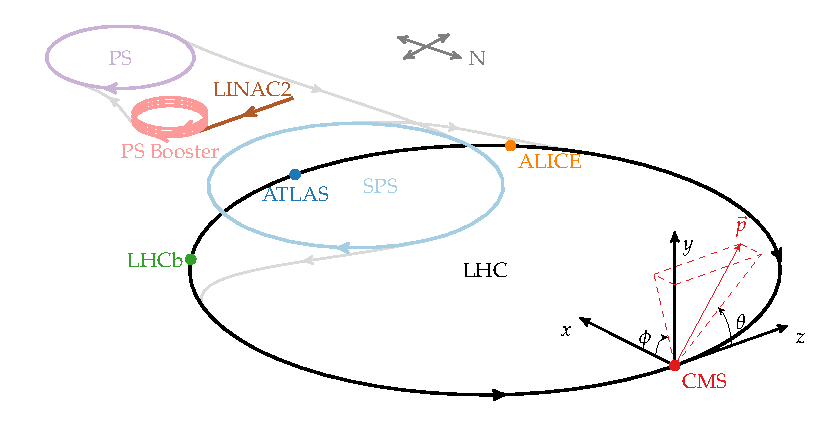
\includegraphics[width =0.9\linewidth]{Figures/Detector/LHC/lhc_complex.pdf}\hfill%               
\caption[The CERN accelerator complex.]{A schematic view of the accelerator chain that services the LHC, known as the CERN accelerator complex. Proton beams are accelerated sequentially by LINAC2, the PS booster, PS, and the SPS, before finally entering the LHC ring where the beam energy reaches 6.5~TeV. The four primary LHC experiments located at interaction points are also shown. The co-ordinate system used by the CMS detector is shown in both cartesian and polar co-ordinates, illustrated for a particle of momentum $\vec{p}$. Note that the size of each component is not to scale, and that the positions serve only as a guide to the real physical location. Figure taken from Ref~\cite{shane_thesis}.}
\label{fig:det_cern_accelerator_complex}
\end{figure}

\subsection{Luminosity}

The LHC has operated in two main phases: Run 1, where data were collected at a centre-of-mass energy of both 7 and 8~TeV, over the period spanning 2009--2013, and Run 2, where data were taken between\footnote{A limited dataset was also collected during 2015, amounting to approximately 2~$\mathrm{fb}^{-1}$} 2016 and 2018 at an increased centre-of-mass energy of 13~TeV. During the Run 2 phase, the LHC surpassed its design instantaneous luminosity, $\mathcal{L}$, reaching $\mathcal{L}=2\times10^{34}$~$\mathrm{cm}^{-2}\mathrm{s}^{-1}$ throughout much of 2018. Operating at a high $\mathcal{L}$ benefits the statistical power of resulting analyses, since the rate of a particular physics process, $n$, is given by the relation

\begin{equation}
\label{eqn:rate_of_proc}
  n=\sigma\mathcal{L},     
\end{equation}

\noindent where $\sigma$ is the cross section for the process. A high centre-of-mass energy can also benefit analyses of rare physics processes, including Higgs boson production, where the cross section scales with increasing $\sqrt{s}$.
Integrating Eqn.~\ref{eqn:rate_of_proc} over the data taking period gives the total number of events for the given physics process, $N=\sigma L$, where $L$ is the integrated luminosity, a measure of the dataset size that is dependent only on the LHC beam parameters and operating time.
Figure~\ref{fig:detector_lumi_pileup} shows the cumulative integrated luminosity delivered to the CMS experiment by the LHC for each year of the Run 2 data taking period, amounting to 159.3~$\mathrm{fb}^{-1}$ in total.
Due to inefficiencies and quality requirements during data collection, the size of the dataset recorded at CMS is approximately 15\% smaller than that delivered by the LHC.

Although an increased instantaneous luminosity allows for collection of larger datasets, it poses challenges elsewhere, including an increased rate of inelastic pp collisions known as \textit{pileup} (PU). Pileup events occur concurrently with rarer processes of interest, and must therefore be separated during many physics analyses, particularly those using jets. Figure~\ref{fig:detector_lumi_pileup} shows the distribution of PU interactions per bunch crossing for each year of the Run 2 data taking period. As the instantaneous luminosity was raised, the average number of PU interactions per bunch crossing increased from 27 in 2016, to 38 and 37 in 2017 and 2018, respectively. 

\begin{figure}[htbp!]
\centering
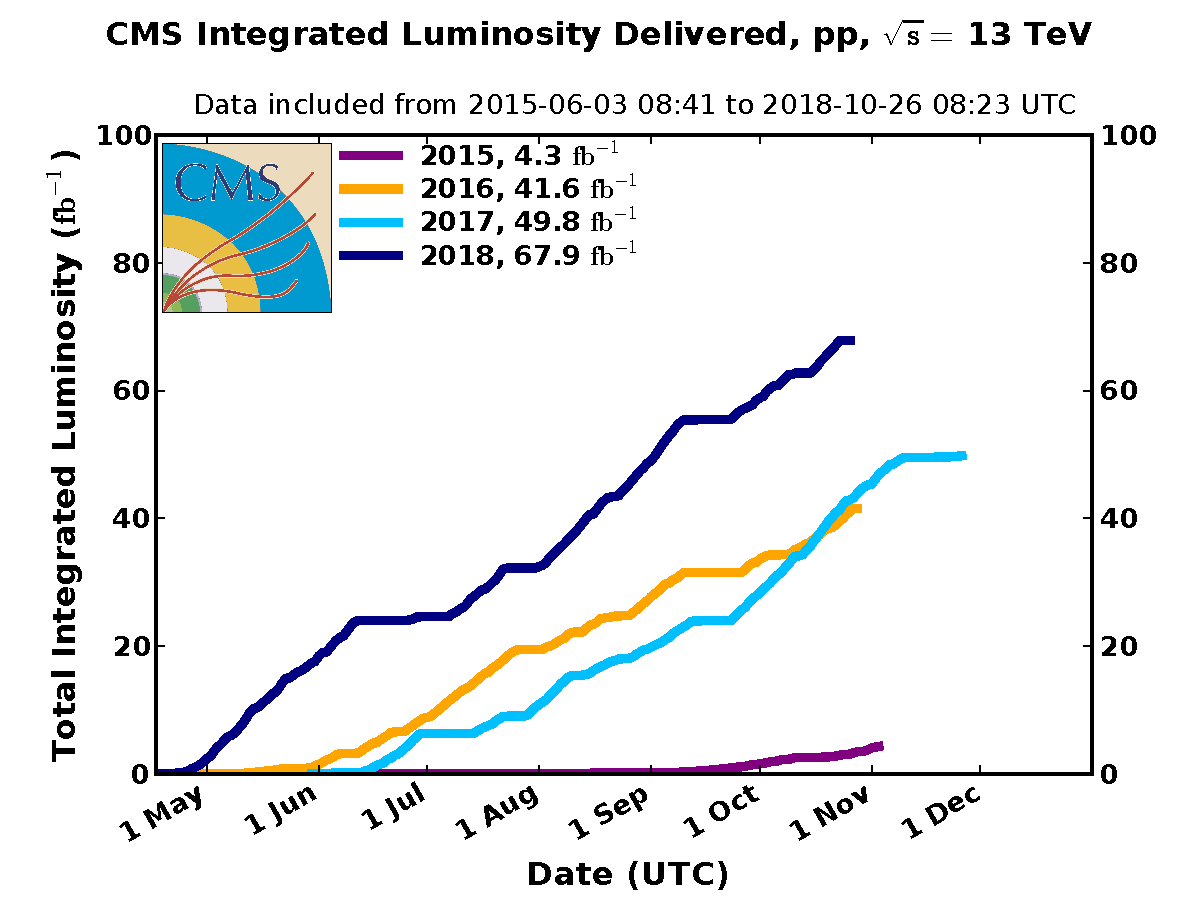
\includegraphics[trim={0cm 0cm 0cm 1.96cm}, clip, width=0.49\linewidth]{Figures/Detector/LHC/int_lumi_cumulative_pp_2_run2.pdf}\hfill%
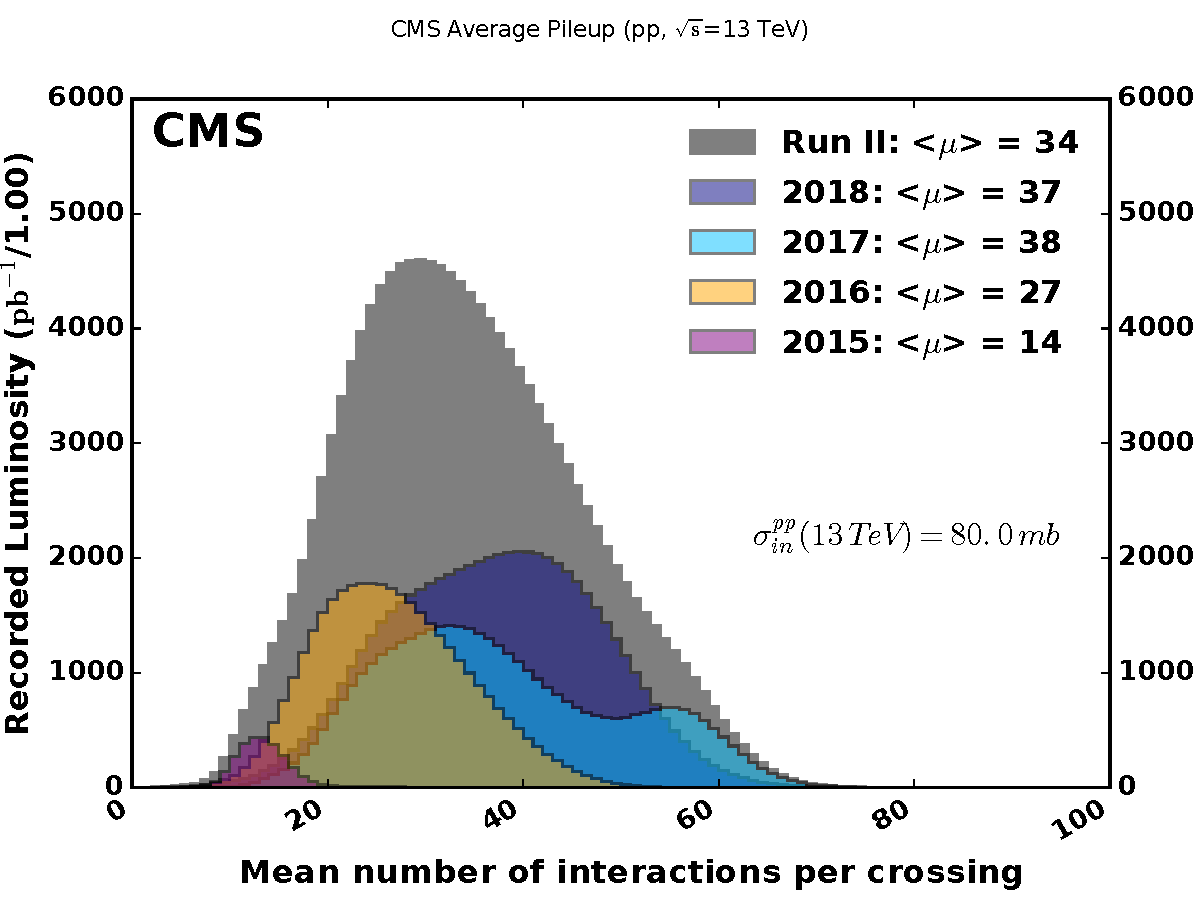
\includegraphics[trim={0cm -0.3cm 0cm 1.5cm}, clip, width=0.46\linewidth]{Figures/Detector/LHC/pileup_allYears_run2.pdf}\hfill% 
\caption[The integrated luminosity delivered to CMS, and the average number of PU interactions per bunch crossing.]{Left: the cumulative integrated luminosity delivered to the CMS experiment per month, shown for the years 2015--2018. Right: the distribution of the number of PU interactions per bunch crossing, between the years 2015 and 2018. The average number of PU interactions increases with the instantaneous luminosity of the LHC; for the total Run 2 period (2016--2018), the average number is 34. Figures are taken from Ref~\cite{CMSLumiPublic}.}
\label{fig:detector_lumi_pileup}
\end{figure}



%%%%%%%%%%%%%%%%%%%%%%%%%%%%%%%%%%%%%%%%%%%%%%%%%%%%%%%%%%%%%

\section{The CMS detector}

The CMS detector is one of two general-purpose physics apparatus on the LHC ring, designed to measure the products of particle collisions. It has a cylindrical shape, measuring over 28~m in length and 15.0~m in diameter, and weighs approximately 14,000 tonnes. The detector is composed of many subsystems, each responsible for measuring different aspects of collisions. The component closest to the beamline is the silicon tracker, followed by the electromagnetic and hadronic calorimeter (ECAL and HCAL, respectively) systems. These are enclosed by the superconducting solenoid, a central feature of the detector which drives the overall design. The most exterior components are the muon detection systems which are interleaved with the return yoke of the magnet.

Each component is required to operate within the high luminosity LHC environment, posing significant constraints on many aspects of the detector design. Materials must be radiation tolerant in order to withstand high particle fluences, while also providing a readout fast enough to contend with the 25~ns collision window. In addition, the detector instrumentation must be granular enough to provide fine spatial and temporal measurements within the high occupancy environment. Further to the operating constraints, the CMS detector should facilitate a diverse physics programme, requiring sensitivity to a wide range of particles and other objects used in physics analyses (\textit{physics objects}). This includes making precise tests of the SM, such as measurements of the Higgs boson and its interactions with other particles, as well as performing searches for dark matter and other processes not predicted in the SM. To achieve these physics objectives, CMS was designed with following key considerations: 

\begin{itemize}
    \item \textit{Muon identification and momentum resolution:} over a  wide  range  of  momenta and angles, muons should be identified with high efficiency and be well measured. This includes good invariant mass resolution for dimuon pairs, and a requirement to unambiguously determine the muon charge. These considerations are particularly important for Higgs boson measurements in the $\mathrm{H}\rightarrow \mathrm{ZZ}^{*}$ decay channels.
    %(sigma(mee) $\approx$1\% at 100 GeV)
    
    \item \textit{Charged particle momentum resolution:} charged particles must be reconstructed with a high efficiency, and their momentum should be well measured by the tracker components.  The efficiency for triggering on, and subsequent offline tagging of, $\tau$ leptons and jets originating from $\mathrm{b}$ quarks should be good. %requiring pixel detectors close to the interaction region because decay length is short
    
    \item \textit{Energy resolution for EM objects}: a wide coverage that should provide good invariant mass resolution for diphoton and dielectron objects. These requirements directly impact the \Hee decay channel studied within this thesis.
    %again, sigma(mee) $\approx$1\%  at  100 GeV
    
    \item \textit{Missing transverse energy resolution}: missing energy is an expected signature in many BSM theories, including supersymmetric extensions to the SM. Measuring the missing energy with high resolution requires hadronic calorimeters with large geometric coverage and granular instrumentation.
    %also want dijet objects to be measured with good mass
\end{itemize}

%Each sub-detector in CMS, discussed in the following Sections, contributes to meeting the above design requirements.
\noindent A schematic of the CMS detector, including a brief description of each component, is shown in Figure~\ref{fig:cms_detector}.

\begin{figure}[htbp!]
\centering
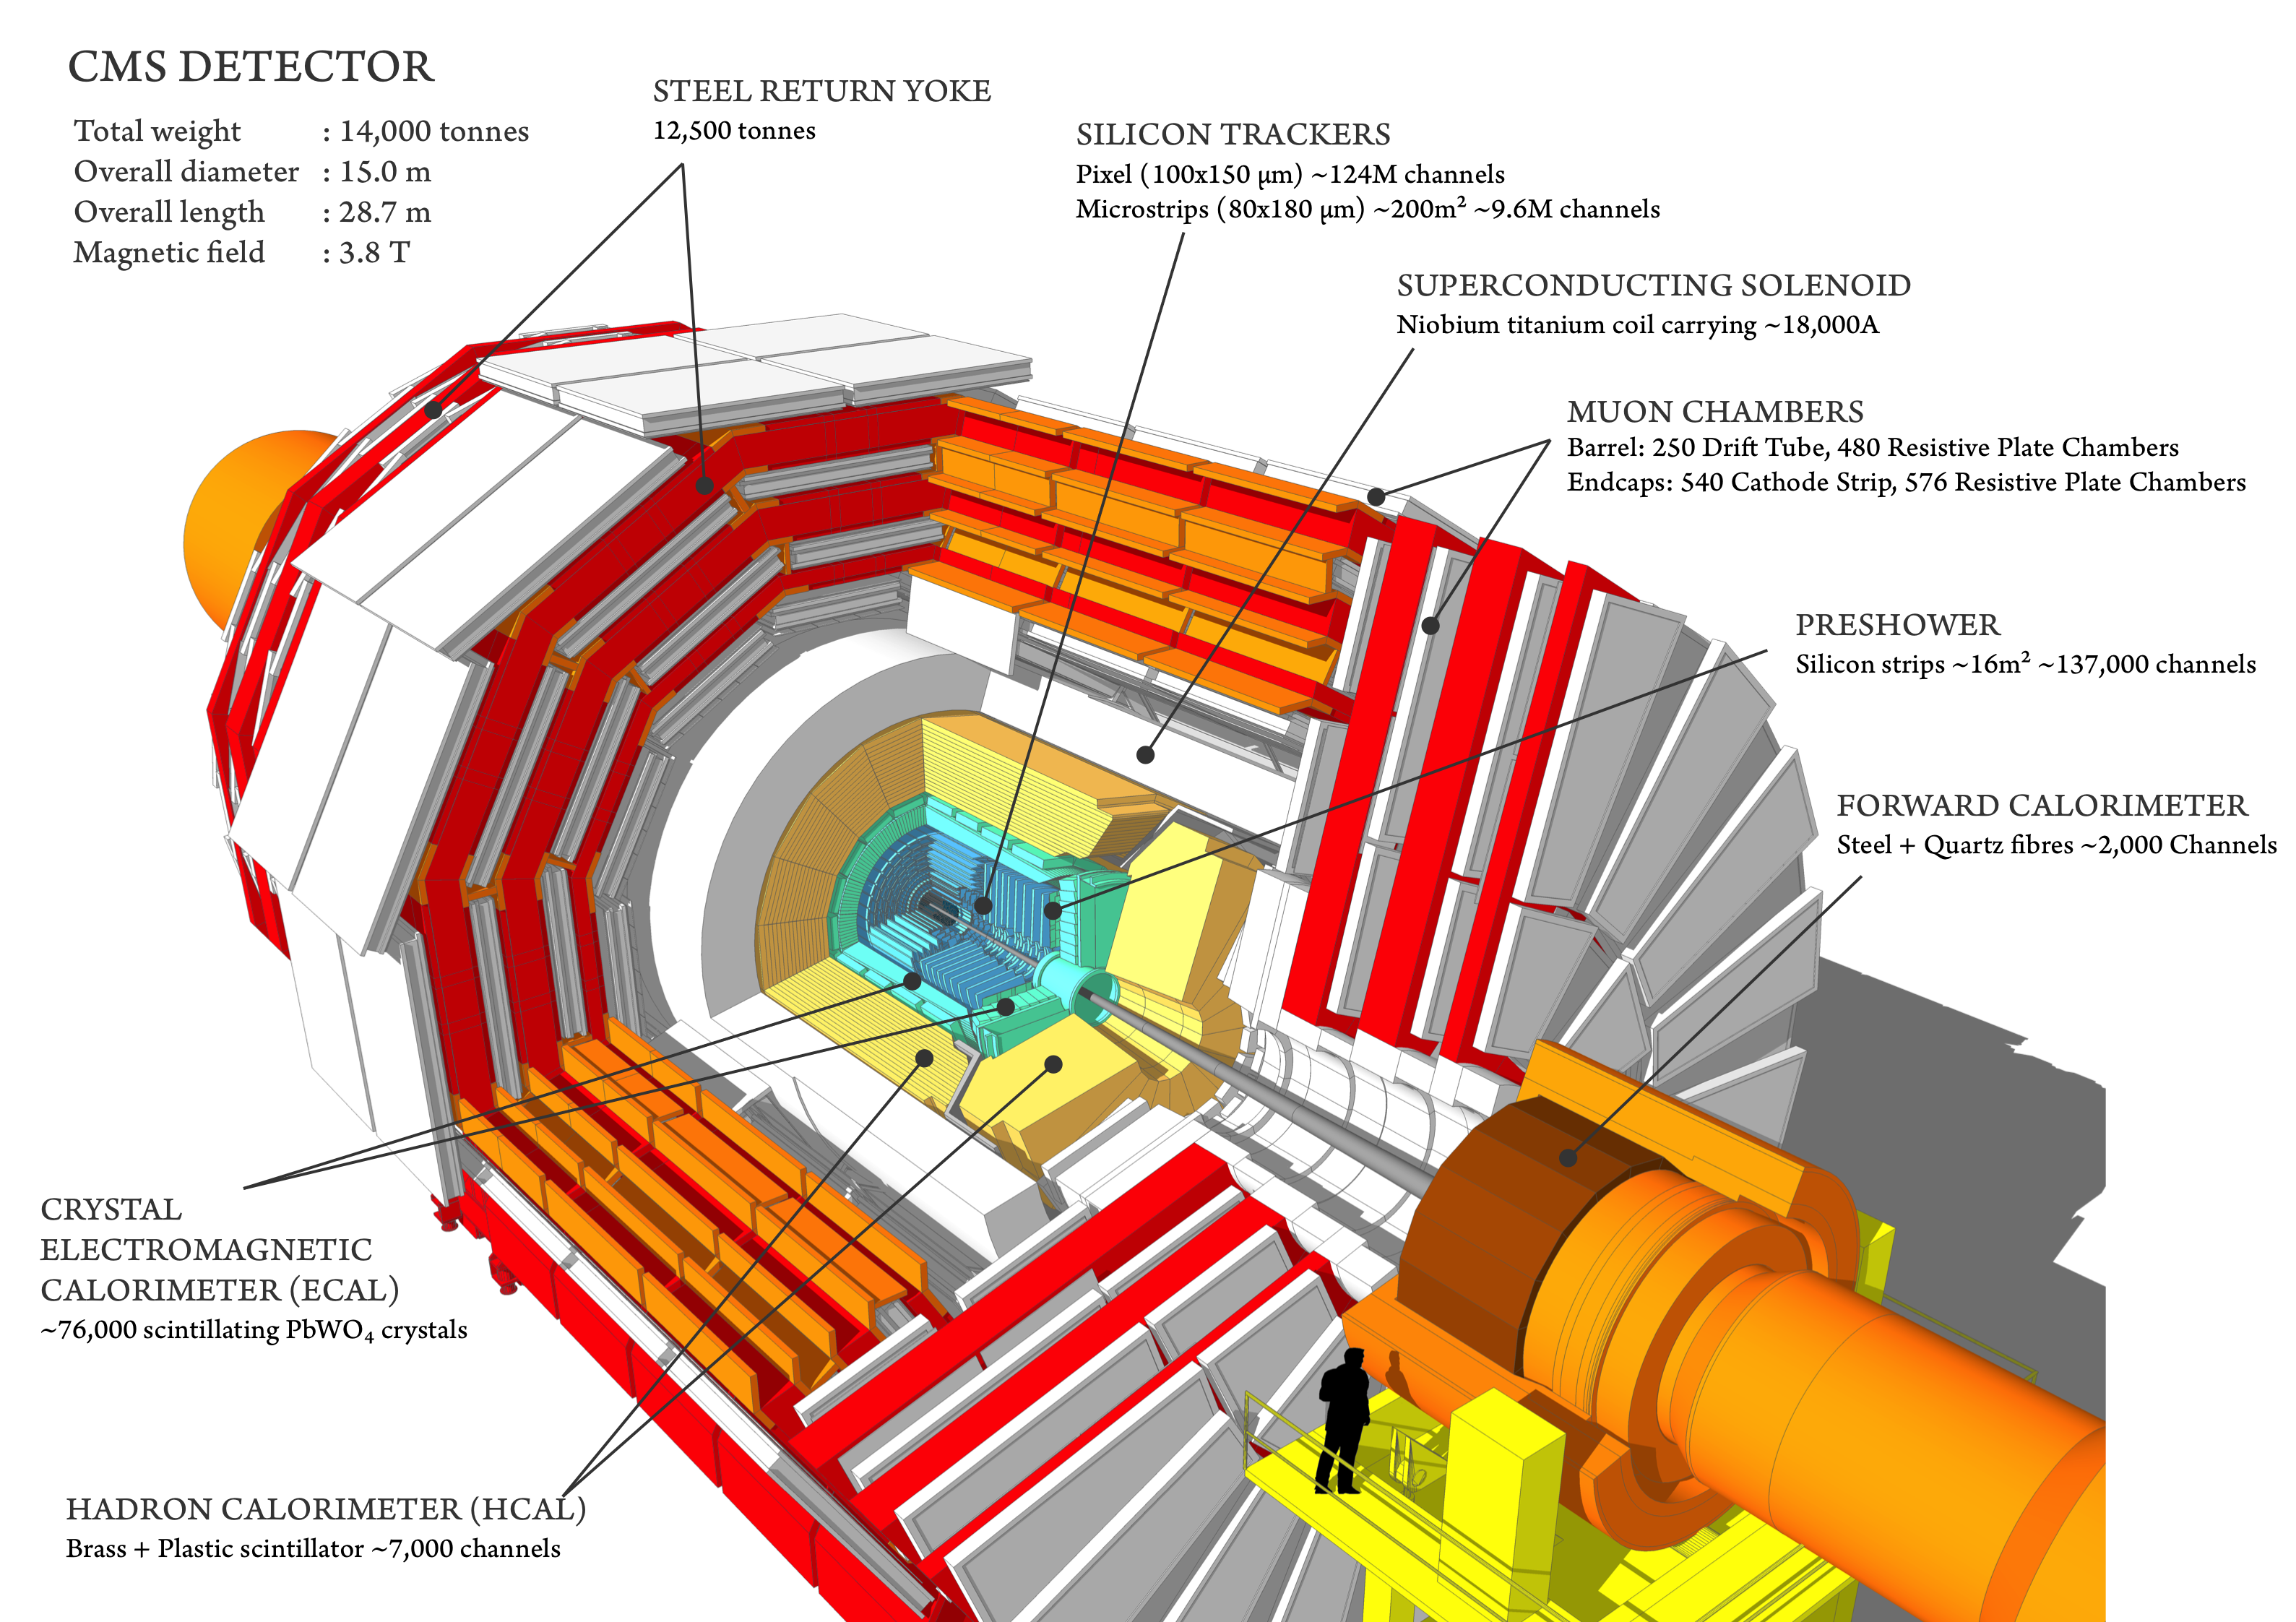
\includegraphics[width =0.92\linewidth]{Figures/Detector/CMS/CMS_cut_away.png}
\caption[The CMS detector.]{A schematic of the CMS detector, where a section is cut away in order to expose each subsystem. Figure taken from Ref~\cite{SketchUp}.}
\label{fig:cms_detector}
\end{figure}

\subsection{Co-ordinate system}

The co-ordinate system adopted by CMS has the origin centred at the collision point. The $z$-axis points in the longitudinal direction along the beamline, the $x$-axis points radially inward to the centre of the LHC, and the $y$-axis points vertically upward. For convenience, quantities are also expressed in a cylindrical co-ordinate system, with particle directions described by the quantities $\eta$ and $\phi$. The quantity $\eta$, referred to as the pseudorapidity, is defined as $\eta=-\ln\left[\tan\left(\theta/2\right)\right]$, and used as a measure of the polar angle relative to the beam axis, $\theta$. Particles with high $\eta$ values are described as \textit{forward}. The quantity $\phi$ is the azimuthal angle in the $x$-$y$ plane. The distance measure in $\eta$-$\phi$ space, $\Delta R$, is also used to describe, for example, the separation of two particles, defined as $\Delta R= \sqrt{ \Delta \eta^{2} + \Delta \phi^{2}}$. Other common quantities include the component of momentum (energy) in the direction transverse to the beamline, \pt ($E_{T}$), and the magnitude of the negative vector sum of particle momentum in the same transverse plane, \met. The CMS co-ordinate system is summarised in Figure~\ref{fig:det_cern_accelerator_complex}.
%these variables capture the three d.o.f.'s in pp collisions: the two Bjorken x's, and the energy.
%pseduorapidity is the rapidity under approximation of negligible particle mass (p275 Thompson)

\subsection{Tracker}

The tracking system is the innermost component of the CMS detector, aiming to precisely determine the trajectories of charged particles passing through its coverage. In addition, the tracker must accurately reconstruct the primary vertex of the hard scattering process, as well as locating any decay vertices of secondary particles, such as those resulting from B hadron decays. To perform these tasks at the high instantaneous luminosity and bunch crossing frequency of the LHC, the tracker components must be instrumented granularly, with extremely fast readout capabilities. Such requirements imply a high density of detector electronics with associated cooling systems, significantly increasing the material budget. However, a larger mass of instrumented material results in undesirable interactions that may adversely affect the physics performance of the detector. These include multiple scattering events and bremsstrahlung radiation, which degrade the tracker momentum resolution. Proximity to the beam pipe also necessitates the tracker to be built using radiation hard materials. As a compromise between the above constraints, the tracker is instrumented solely with silicon-based technologies, which provide good spatial and temporal resolution at a low material budget, while also tolerating a high radiation environment. 

%PIXEL DETECTOR UPGRADE AND SUBSEQUENT SPECS 
The CMS tracker has cylindrical geometry and provides tracking capabilities up to $|\eta|\;<2.5$.
The system provides measurements along the charged particle trajectory, known as \textit{hits}, which seed the track reconstruction algorithms presented in chapter~\ref{chap:eventCategorisation}.
It is composed of two distinct components: a silicon pixel detector, which extends to a radial distance of 20~cm, and a silicon strip detector which covers the remaining volume out to a radius of 1.1~m. 
The original pixel detector, which was designed to operate for ten years, was instrumented with 66 million sensors, each measuring $100~\mu\mathrm{m}\times150~\mu\mathrm{m}$. Closest to the interaction point, the sensors were organised into three cylindrical layers situated at radii of 4.4, 7.3, and 10.2~cm. Two additional pixel endcap detectors arranged in disks sat either side of this central module at longitudinal distances of $\pm34.5$ and $\pm46.5$~cm, extending the $\eta$ coverage. During the technical pause scheduled at the end of 2016, the pixel tracking system was upgraded, in expectation of greater particle fluence during the remainder of Run 2~\cite{CMS_phase1_tracker_upgrade}. The upgrade aimed to mitigate radiation damage associated with the increased luminosity environment which can reduce the charge collection efficiency of modules, leading to reduced spatial resolution, particularly for components closest to the beamline. The associated increase in number of pileup interactions is also detrimental to the physics performance, resulting in lower tracking efficiencies. The upgrade improved the granularity of readout components, with the number of cylindrical layers increased by one. This allows for four spatial measurements along the charged particle trajectory in the barrel region, at radii of 2.9, 6.8, 10.1, and 10.6~cm. An additional silicon disk was also added to each endcap section, such that the endcaps provide measurements at longitudinal distances of $\pm$29.1, $\pm$39.6, and $\pm$51.6~cm. These modifications result in an excellent spatial resolution of around 13 and 20~$\mu\mathrm{m}$ in the transverse and longitudinal directions respectively. The new components are lower mass in order to maintain a reasonable material budget, whilst also more radiation hard than their predecessors. A schematic of the upgraded tracker layout is shown in Figure~\ref{fig:cms_tracker}. %data loss was from readout buffers than were full so cant accept any more info. Note than after the upgrade, the number of readout channels was more like 123 million.

\begin{figure}[htbp!]
\centering
\includegraphics[width =0.92\linewidth]{Figures/Detector/CMS/tracker_run2_upgraded.pdf}\hfill%               
\caption[The CMS tracking system.]{One quarter of the CMS tracking system, shown in the $r$-$z$ view. Components of the silicon pixel detector are shown in green, while the strip detectors are coloured in both orange and blue, denoting single-sided and double-sided modules respectively. The silicon pixel detector was upgraded during the technical pause between 2016 and 2017 to account for the expected increase in particle fluence. Figure taken from Ref~\cite{CMS_phase2_tracker_upgrade}.}
\label{fig:cms_tracker}
\end{figure}

%OUTER TRACKER (unchanged)
The outer tracker uses silicon strip technologies, and can be divided into three components. The innermost components are the tracker inner barrel (TIB) and associated endcaps (TIDs), which extend to a radial distance of 55~cm. The TIB consists of four layers of silicon strip sensors, arranged parallel to the beam axis, orthogonal to the three disk layers that comprise each TID. %looks like 8 but the two nearby layers are actually just a single layer (4 times)
Together, the TIB and TID can perform up to four position measurements along a particle trajectory, with a spatial resolution between approximately 20 and 35 $\mu\mathrm{m}$.
Exterior to these components is the tracker outer barrel (TOB), the outermost component, extending to a radius of 116~cm. The TOB consists of six layers, each of which provides an additional measurement along the charged particle trajectory.
Note that the first two layers of the TIB, TIDs, and TOB are also mounted back-to-back with a second silicon strip module, which provides an additional $z$ ($\phi$) measurement in the barrel (endcap) region. Finally, the $\eta$ coverage is extended by two tracker endcaps (TECs), positioned symmetrically about the interaction point, between $z$ co-ordinates of $\pm124~\mathrm{cm}$ and $\pm282~\mathrm{cm}$. 
Each TEC is instrumented with 9 disks, carrying up to seven concentric rings of silicon strip sensors. The first, second, and fifth rings of the TEC are mounted with second silicon sensors, providing further 2D measurements.

With all components combined, the tracker geometry ensures a minimum of 9 hits over the full $\eta$ range, with at least four of them providing two-dimensional measurements. The momentum resolution is $<1\%$ for particles produced centrally ($|\eta|\;<1$) with $\pt \approx 10$~GeV, which is dominated by multiple scattering affects. At higher energies, these effects are significantly reduced; however, the associated tracks experience less curvature in the CMS magnetic field, resulting in a worsening in \pt resolution to $<2\%$ for particles with $\pt \approx 100$~GeV and $|\eta|\;<1$.

\subsection{Electromagnetic calorimeter}


%general overview of the structure and overall motivation/objective of the ECAL
The CMS electromagnetic calorimeter is a homogeneous calorimeter designed to measure the energy deposits of particles that interact electromagnetically. Alongside the tracker, it is an important component in reconstructing and identifying electrons produced in the \Hee decay.

The ECAL, shown in Figure~\ref{fig:cms_ecal}, is comprised of a cylindrical barrel section (EB) which spans the pseudorapidity range $|\eta|\;<1.48$, enclosed by two endcaps (EE) that increase the angular coverage to $|\eta|\;<3.0$. Both the EB and EE are instrumented with lead tungstate  ($\mathrm{PbWO}_{4}$) crystals that produce scintillation light when incident with photons or electrons. The light is collected by photodetectors that convert the response to a voltage, proportional to the energy of the incident particle. Each crystal in the EB (EE) has a frontal area of $22\times22~\mathrm{mm}^2$ ($28.6\times28.6~\mathrm{mm}^2$), and is 230~mm (220~mm) in length. The transverse size of each crystal is comparable to the typical width of an EM shower deposited in $\mathrm{PbWO}_{4}$, facilitating photon and electron identification using properties of the (resolvable) shower shape. The barrel region consists of 61,200 such crystals, which are grouped into 36 supermodules that each cover half the EB length and 20$^{\circ}$ in $\phi$. The axis of crystals inside a supermodule is rotated by a 3$^{\circ}$ angle in both $\eta$ and $\phi$ with respect to the interaction point, in order to avoid particles passing entirely through a gap region. The endcaps, which are divided into two semi-circular halves, or \textit{dee's}, each hold a further 3662 crystals arranged into $5\times5$ groups of so-called \textit{supercrystals}. Finally, preshower detectors (ES) are placed in front of each EE region, covering the range $1.65<|\eta|\;<2.6$. 
Each ES contains two layers of lead absorber designed to initiate EM showers, instrumented with granular silicon strip modules used to improve the misidentification of photons from $\pi^{0}\rightarrow \gamma\gamma$ decays.
% %high eta = smaller angle between photons so can mistake for one photon that is later confused with prompt gamma. Lead abosrber also encourages shower initiation.
% could have had a preshower in the barrel, but went for a larger tracker volume instead

\begin{figure}[htbp!]
\centering
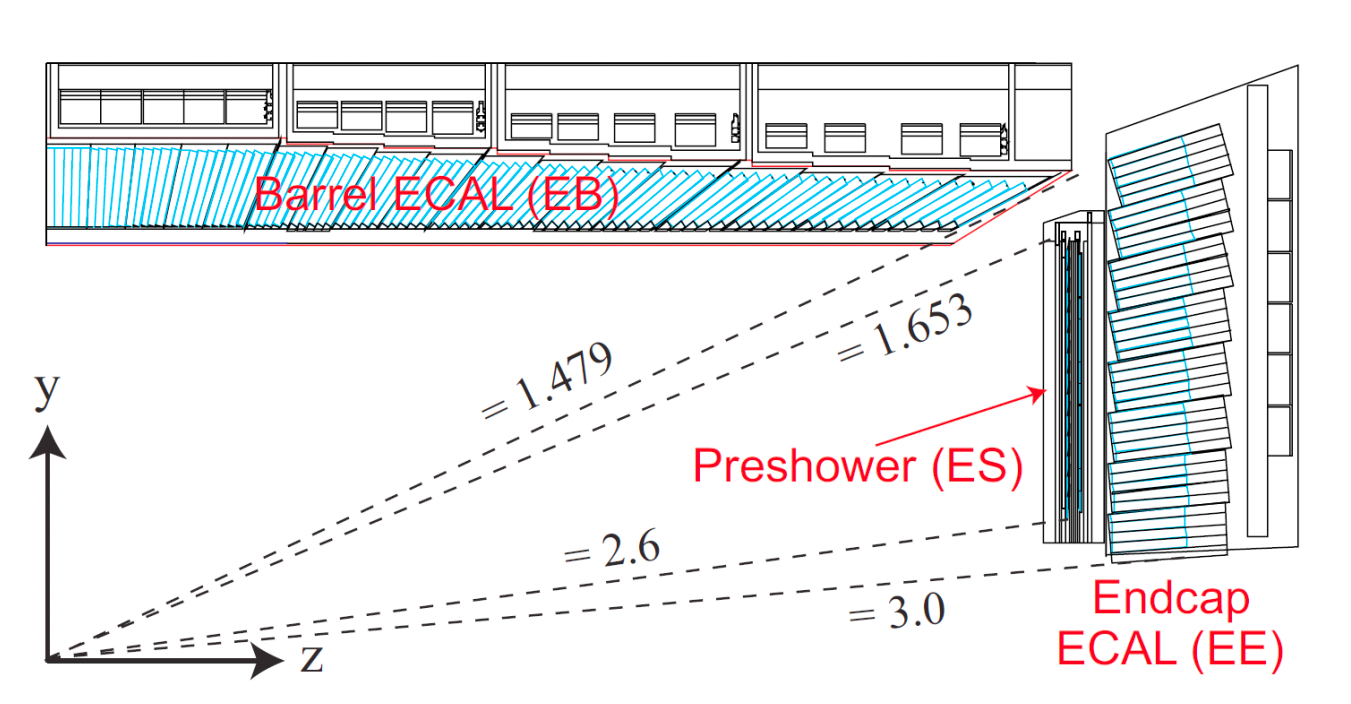
\includegraphics[width =0.8\linewidth]{Figures/Detector/CMS/ECAL_quadrant.png}\hfill%     
\caption[The CMS electromagnetic calorimeter.]{One quarter of the CMS ECAL, annotated with the pseudorapidity coverage of the EB, EE, and ES. Figure taken from Ref~\cite{CMS_ECAL_extra_info}.}
\label{fig:cms_ecal}
\end{figure}

The choice of lead tungstate crystal is driven by the material's high density (8.28~$\mathrm{g/cm}^{3}$) and short radiation length\footnote{A radiation length is defined as the mean distance over which a high energy electron will lose all but $1/e$ of its initial energy, due primarily to bremsstrahlung radiation.}%hence the high energy
, $X_{0}$, (0.89~cm) which allow for a compact design that provides good containment of EM showers over the full 25.8~$X_0$ longitudinal length. A small Moli\'ere radius\footnote{A Moli\'ere radius characterises the lateral shower containment, and is defined as the radius of a cylinder containing on average 90\% of the deposited shower energy.} (2.2~cm) also inhibits shower spreading in the transverse plane. The LHC operating conditions pose further requirements on the crystal properties, including a response time compatible with the 40~MHz bunch crossing frequency, and adequate radiation hardness. The $\mathrm{PbWO}_{4}$ crystals emit 80\% of light within the required 25~ns collision window, and are reasonably tolerant to radiation damage; however, over time, the exposure to high particle fluences causes the crystals to transmit less light. This effect can be at the level of ${\approx}10\%$ for crystals positioned at high $\eta$, and must therefore be monitored and corrected for by measuring the optical transparency using laser light.
%The RMS for the crystal light is nearly 10%, so the response of crystal has to be calibrated against the rest using cosmic rays, test beam, physisc events, etc.

The light yield from $\mathrm{PbWO}_{4}$ crystals is relatively low and must be amplified by on-detector electronics. To this end, each crystal in the barrel is mounted with an avalanche photodiode, responsible for both collecting and amplifying scintillation light. In the endcap region, where the particle fluence is significantly higher, crystals are instrumented with vacuum phototriodes, capable of operating within the high axial magnetic field. The photodetectors produce approximately 4,500 photoelectrons per GeV of energy deposited, which are converted to digital format using analog-to-digital (ADC) converters. The digitised amplitudes are buffered while awaiting trigger decision, before being transferred to off-detector electronics.
%check these are similar to your typical "avalanche" PMT
% The photodetectors produce approximately 4,500 photoelectrons per GeV of energy deposited, which are converted to digital format using analog-to-digital (ADC) converters
%The ammount of energy in the shower can be obtained from the pulse shape.

%Energy resolution (for energies below 500~GeV before leakage becomes singifcant)
The energy resolution of the CMS ECAL is particularly important for the \Hee analysis, where resolving the narrow signal peak in the dielectron mass distribution increases the signal-to-background ratio. For the majority of particle energies at the LHC, the intrinsic energy resolution can be parameterised by

\begin{equation}
    \left( \frac{\sigma}{E} \right)^2 =  \left( \frac{S}{\sqrt{E}} \right)^2 + \left( \frac{N}{E} \right)^2 + C^{2},
\end{equation}

\noindent where $S$ is the stochastic term, $N$ is the noise term, and $C$ is the constant term.
Each coefficient is fit to data collected during test beams; for energies in GeV, characteristic values of S=2.8\%, N=12\%, and C=0.3\% are obtained~\cite{CMS}. 
%S: shower development is stochastic in nature so this is intrinsic "Poisson" error on number of particles in the shower
%N: readout electronic noise, effects of cosmics, out of time pilueup overlapping noise, etc.
%C: everything else: imperfections is calorimeter construction e.g. dimensions, fluctuations in energy containment, energy leakage, effect of dead material housing the components etc.


%Final piece about inter calibration of crystals
Showers resulting from both electrons and photons are typically spread over several ECAL crystals. Therefore, in order to build candidate EM objects, these energy deposits must be combined into so-called \textit{superclusters} (SC), from which an energy can be estimated. The reconstructed energy~\cite{CMS_ECAL_extra_info} of an electron or photon SC can be described using

\begin{equation}
\label{eqn:egamma_reco_energy}
    E_{e/\gamma} = F_{e/\gamma} \cdot \left[ G\sum_{i}S_{i}(t)C_{i}A_{i}  + E_{\mathrm{ES}}\right],
\end{equation}

\noindent where, firstly, the digitised signal amplitudes ($A_{i}$) are summed over each of the $i$ channels in the SC, weighted by coefficients that correct for time ($S_{i}(t)$) and channel ($C_{i}$) dependent changes in response. The resulting amplitude is multiplied by the ADC-to-GeV conversion factor (G), and summed with any associated energy deposited in the preshower plates ($E_{\mathrm{ES}}$). Lastly, any residual effects from imperfect clustering, upstream material, and detector geometry are accounted for by a global correction factor ($F_{e/\gamma}$), estimated using a series of multivariate regressions. The procedure to obtain $F_{e/\gamma}$ is described in chapter~\ref{chap:eventCategorisation}, where it is also validated for the \Hee analysis.
%C_{i}: want equal response from each channel. Computed using known masses of pi zero and eta decays to two photons, and the azimuthal invariance. Also use comsic muon to do this which deposit constitent ammount of energy.
%G: measured by using the known Z-mass resonance. Its just like any physics detector standard candle calibration 
%F: obtained from the energy regression

\subsection{Hadronic calorimeter}

The Hadronic calorimeter is a sampling calorimeter, placed between the ECAL and inner extent of the magnet coil~\cite{CMS,HCAL}. It is designed primarily to measure the energy deposits of charged and neutral hadrons, but also plays an important role in measurements of \met. Figure~\ref{fig:cms_hcal} shows the layout of each sub-component in the HCAL. It is comprised of a barrel region (HB) which extends to a radius of 2.95~m, two endcaps (HE), and a forward region (HF) that increase the angular coverage up to large pseudorapidities.  

Modules in the HB are arranged into two half barrels consisting of 18 azimuthal wedges, placed either side of the interaction point, and covering the range $|\eta|\;<1.3$. The wedges are constructed using brass absorber plates designed to initiate hadronic showers. Brass is chosen for its large nuclear interaction length\footnote{A nuclear interaction length is defined as the mean distance travelled by a hadron before undergoing an inelastic nuclear interaction.}, $\lambda_{I}$, (16.4~cm) which allows for good shower containment within the HCAL volume, and for its tolerance to a high radiation environment. In total, the absorber contains between 5.8 and 10.6~$\lambda_{I}$ of material, depending on the $\eta$ angle. Each absorber wedge is interleaved with trays of silicon tiles, divided into 16 sectors based on $\eta$. This results in approximately 70,000 tiles in total, with a segmentation of 0.087 in both $\eta$ and $\phi$. The tiles produce scintillation light which is read out by wavelength-shifting plastic fibres and used to infer the energy of the incident hadron.
%PMTs also amplify the signal

Beyond the solenoid sits the most exterior component of the HCAL: the outer hadronic calorimeter (HO). The HO uses the solenoid and iron return yoke as the absorber material, extending the number of nuclear interaction lengths by 2--3. Without this additional material, space constraints imposed by the magnet would result in an inadequate amount of stopping power within the central region, impacting the energy resolution for late-starting hadronic showers and \met measurements. The HO uses the same plastic scintillator technology readout, positioned within the rings of the magnet return yoke, with similar segmentation to the HB.

The HCAL endcaps cover a substantial portion of the pseudorapidity range, extending out to $|\eta|\;<3$. Given the proximity to the beamline, the HE must be tolerant to large particle fluences, and contain as many nuclear interaction lengths as possible in order to contain hadronic showers. These considerations lead to brass also being chosen as the absorber, resulting in approximately 10~$\lambda_{I}$ of material when including the EE. Silicon scintillator tiles instrument the absorber with a granularity equivalent to the HB for $|\eta|\;<1.6$. For angles closer to the beamline, this segmentation reduces to 0.17 in both $\eta$ and $\phi$.

The final components of the HCAL system are the forward calorimeters, positioned at $z=\pm11.2~\mathrm{m}$ downstream of the interaction point. These components experience extremely high particle fluxes; on average, the energy deposition in the two HF detectors is almost 800~GeV per interaction, compared to around 100~GeV for the rest of the detector. This environment poses considerable challenges to calorimetery and is the driving design requirement for the HF. To meet these challenges, the HF uses a steel absorber material, with grooves instrumented by radiation hard quartz fibres for readout. The fibres produce Cerenkov light which is collected by photomultiplier tubes. Over 1000~km of fibres are arranged parallel to the absorbers, and are divided into two lengths --- a longer fibre runs the full length of the HF, while shorter fibres start at a depth of 22~cm from the front face. This arrangement allows for separation of EM and hadronic showers, which penetrate the material to differing depths. The HF calorimeters play an important role in reconstructing the VBF \Hee production mode, where the Higgs boson is produced in association with two forward jets.
%EM showers are contained in early part of HF, whereas Hadronic showers deposit energy equally throughout

\begin{figure}[htbp!]
\centering
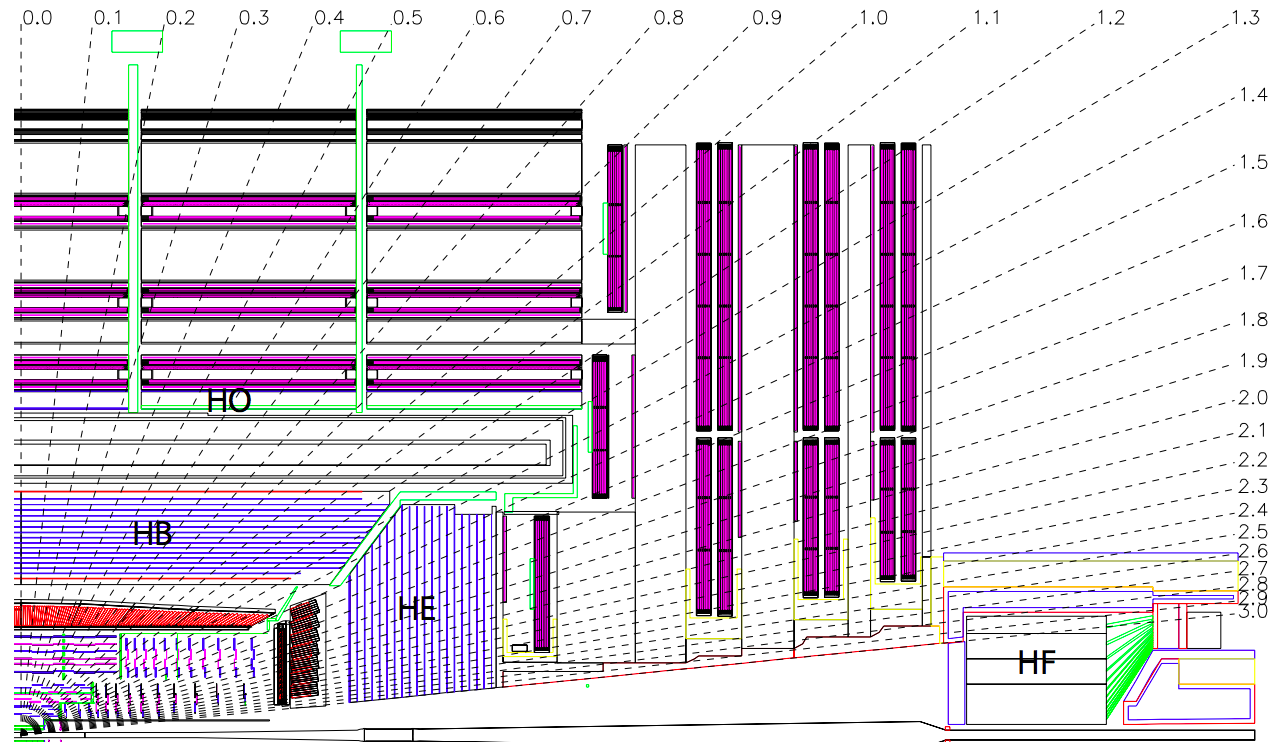
\includegraphics[width =0.75\linewidth]{Figures/Detector/CMS/HCAL_quadrant.png}\hfill \caption[The CMS hadronic calorimeter.]{A quadrant of the CMS hadronic calorimeter, with the primary four regions labelled (HB, HE, HO, HF). Various pseudorapidity angles are also shown by the dashed lines. Figure taken from Ref~\cite{CMS}.}
\label{fig:cms_hcal}
\end{figure}

\subsection{Solenoid}

The central feature of the CMS detector is a 13~m long, 6~m (inner) diameter superconducting solenoid, cooled to a temperature of 4.5$~\mathrm{K}$, and storing an energy of 2.6~GJ at full operating current. The solenoid produces a strong magnetic field of 3.8~T, which greatly benefits the charge assignment efficiency and measurements of the momentum of highly energetic charged particles. These particles bend under the field's influence, allowing the momentum and charge to be determined from the radius and direction of track curvature, respectively. The magnetic flux is confined to the volume of the detector by the steel return yoke, which at 10,000 tonnes, comprises the majority of the CMS detector mass.

\subsection{Muon chambers}

Precise muon reconstruction has been a key physics objective for CMS from its earliest design stages, since muonic final states are expected for many physics processes of interest, including the $\mathrm{H}\rightarrow \mathrm{ZZ}^{*} \rightarrow 4\mu$ Higgs boson decay channel. Muons traverse the CMS apparatus relatively unimpeded, leaving deposits in the tracker and calorimetry systems only through ionisation processes. A dedicated muon tracking system is built into the return yoke for the CMS magnet, designed to extend tracking measurements several metres beyond the interaction point. This system aims to reconstruct the muon charge and momentum over the entire kinematic profile expected at the LHC. It consists of a barrel (MB) and two endcap regions (ME), instrumented with three gaseous detector types. In a typical gas detector, as a charged particle passes through the active volume, atomic nuclei are ionised, creating electron-ion pairs along the particle path. A strong electric field is applied across the chamber, causing a drift of the liberated electrons towards a wire anode. During this drift, an avalanche of subsequent gas ionisations take place, resulting in a measurable charge reaching the anode. The charge pulse across each each anode can then be used to infer the position of the incident particle.
The exact choice of gaseous technology varies with $\eta$, motivated by the expected muon flux, the neutron-induced background, and the local properties of the magnetic field. 
%ions are too heavy to drift considerably. DTs also measure the time between arrival pulses on wires; knowing the electron drift time can give information on how far from the wire the particle passed through the gas
 
In the MB, drift tube (DT) chambers provide tracking capabilities over the range $|\eta|\;<1.2$. The DTs use a mixture of Ar and CO$_{2}$ gases, and are organised into four overlapping stations interspersed throughout the return plates. Each station contains four chambers that measure muon co-ordinates in the $\phi$ direction, and four that provide a measurement of $z$ co-ordinates. In the two endcap regions, the muon system uses cathode strip chambers (CSCs) which provide a fast response time and radiation resistance suitable for the increased particle fluence. Four stations of CSCs instrument each endcap, arranged perpendicular to the beamline, and provide coverage for muons produced between $0.9<|\eta|\;<2.4$. Both the MB and ME regions are also instrumented with resistive plate chambers (RPCs) that operate independently. The RPCs produce a fast response allowing for improved timing resolution that is used to inform the trigger decision. The additional position measurements also help to resolve ambiguities when attempting to form tracks from multiple hits in a single chamber. %why is rate higher in muon forward region, assume PU doesnt go out that far?

Overall, the efficiency to reconstruct and identify muons is greater than 96\%  over the full $\eta$ range. 




\subsection{Trigger}

Given that each 25~ns LHC beam crossing generates approximately 1~Mb of data, recording information from every event would result in insurmountable data processing and storage challenges. The CMS detector therefore uses a two-level trigger system~\cite{CMS_L1T,HLT} to reduce the recorded event rate to a tolerable level. The first Level-1 Trigger consists of custom electronics, which use coarse data from a subset of detectors in order to reduce the recorded event rate to 100 kHz. The second system is the High-Level Trigger (HLT), implemented in software using a farm of commercial processors. In contrast to the L1T, the HLT has access to the full granularity of the detector readout, which is used to form more complex selection criteria that further reduce the event rate to around 1 kHz.
%so guess electrons and photons in the L1T look the same because the track information is not available

\subsubsection{Level-1 Trigger}

The L1T has to perform a factor of 400 decrease in event rate within a latency of 3.2~$\mu\mathrm{s}$. Inputs to the decision algorithms are therefore restricted to basic information from the muon and calorimeter systems only, with no access to the highly segmented readout from the tracker. At this stage, no effort is made to distinguish photon and electron objects, which produce similar signatures in the ECAL. The coarse information is used to form a list of algorithms, known as \textit{seeds}, which check each event against a set of predetermined criteria known as the trigger \textit{menu}. The menu covers the broad physics programme at CMS, maintaining a high efficiency for signals of potential interest. The seed selection typically applies thresholds to the $\pt$ and $\eta$ of physics objects, which are adjusted such that the total menu rate is within 100~kHz. For the Run 2 \Hee search, the final state contains multiple $e$/$\gamma$ candidates, a signature which is allocated 6.4\% of the total L1T rate~\cite{CMS_L1T}.
%These include, for example, final states with a single electron/photon, multi electron/photon objects, and those with at least one jet, which are allocated 24.8\%, 11.5\%, and 6.4\% of the 100~ kHz bandwidth respectively~\cite{L1T}.

The full event resolution information, including the tracker readout, is buffered until a L1T accept signal is generated, where it is then passed on to the HLT.


\subsubsection{High level Trigger}

Filtering by the HLT uses the full precision of data from the detector in order to reduce the event rate by a factor of 100. The event selection is similar to that used in offline algorithms; physics objects including electrons, muons, and jets, are reconstructed, including information from the tracker, and compared against selection criteria that informs whether an event should be accepted. For the \Hee search, the HLT selection comprises asymmetric thresholds on electron \pt, as well as loose isolation requirements which limit energy deposits nearby the electron candidates. Events passing selection are sent to a separate computing farm for further reconstruction offline, and storage.
%iso is to reduce the probability of electrons in jets being associated with tracks

%%%%%%%%%%%%%%%%%%%%%%%%%%%%%%%%%%%%%%%%%%%%%%%%%%%%%%%%%%%%%%%%%%%%%%%%%%%%
%%%%%%%%%%%%%%%%%%%%%%%%%%%%%%%%%%%%%%%%%%%%%%%%%%%%%%%%%%%%%%%%%%%%%%%%%%%%

\section{The High Granularity Calorimeter Phase-2 upgrade}
\label{sec:HGCAL}

\subsection{The High Luminosity LHC}


With Run 2 of the LHC operation concluded, many upgrade projects for both accelerator and detector components are underway. These upgrades are typically scheduled within so-called \textit{long shutdown} (LS) periods, where the LHC beam is inactive. Amongst other projects, the LS2 period, which has been underway since the end of Run 2 operation in 2018, has prepared the LHC to run at a higher centre-of-mass energy of 13.6~TeV. Such upgrades are in anticipation of Run 3, which will span over mid-2022 to 2024, and bring the total integrated luminosity collected at the CMS detector to approximately 300~$\mathrm{fb}^{-1}$. Beyond Run 3, operation of the LHC with the current beam parameters is of limited interest for physics analyses; in order to improve the statistical precision on measurements by a factor of two, ten more years of operation with the Run 3 conditions would be required. Instead, a major upgrade to the LHC is planned, aiming to achieve a substantially increased instantaneous luminosity of up to $5\times10^{34}~\mathrm{cm}^{-2}\mathrm{s}^{-1}$. The upgraded LHC, known as the High Luminosity LHC (HL-LHC)~\cite{HL_LHC}, will run until the mid-2030's, collecting approximately 3000~$\mathrm{fb}^{-1}$ of data. The considerable increase in luminosity benefits many physics analyses, from precision measurements, to searches for rare and exotic processes. In the Higgs sector, rare interactions will be measured with significantly improved sensitivity, including couplings to the light fermions and the Higgs boson self interaction. The expected precision of the Yukawa couplings to various SM particles projected at the end of the HL-LHC operation is shown in Figure~\ref{fig:cms_high_lumi_couplings}. Measurements of Higgs boson production cross sections, such as those defined in the Simplified Template Cross Section scheme~\cite{YR4}, will also be facilitated with unprecedented resolution, allowing for precise tests of the SM predictions.
%possible through 11-12T magnets, crab cavities (bunch rotation) etc.

The benefits of operating at a higher instantaneous luminosity are, however, accompanied by difficulties elsewhere. The average number of pileup interactions per bunch crossing is expected to increase to around 140, requiring highly segmented detector readouts and sophisticated subtraction techniques to prevent confusion with objects of interest. Furthermore, detector components must be sufficiently resistant to the high radiation levels, given that the expected dose in year one of the HL-LHC operation will be equivalent to that absorbed during the entire LHC operation up to Run 3. In order to preserve the performance of the CMS detector despite the challenging environment, many of the detector subsystems will require upgrading. These Phase-2 upgrades are extensive, including a new highly segmented tracker~\cite{CMS_phase2_tracker_upgrade} that will also inform L1T decisions, upgraded and unified ECAL and HCAL endcap components~\cite{CMS_phase2_HGCAL}, and additional instrumentation of the muon system. 

In this section, the calorimeter endcap upgrade project, known as the High Granularity Calorimeter, will be discussed, with a particular focus on its use within L1T algorithms used to identify electromagnetic objects.

\begin{figure}[htbp!]
\centering
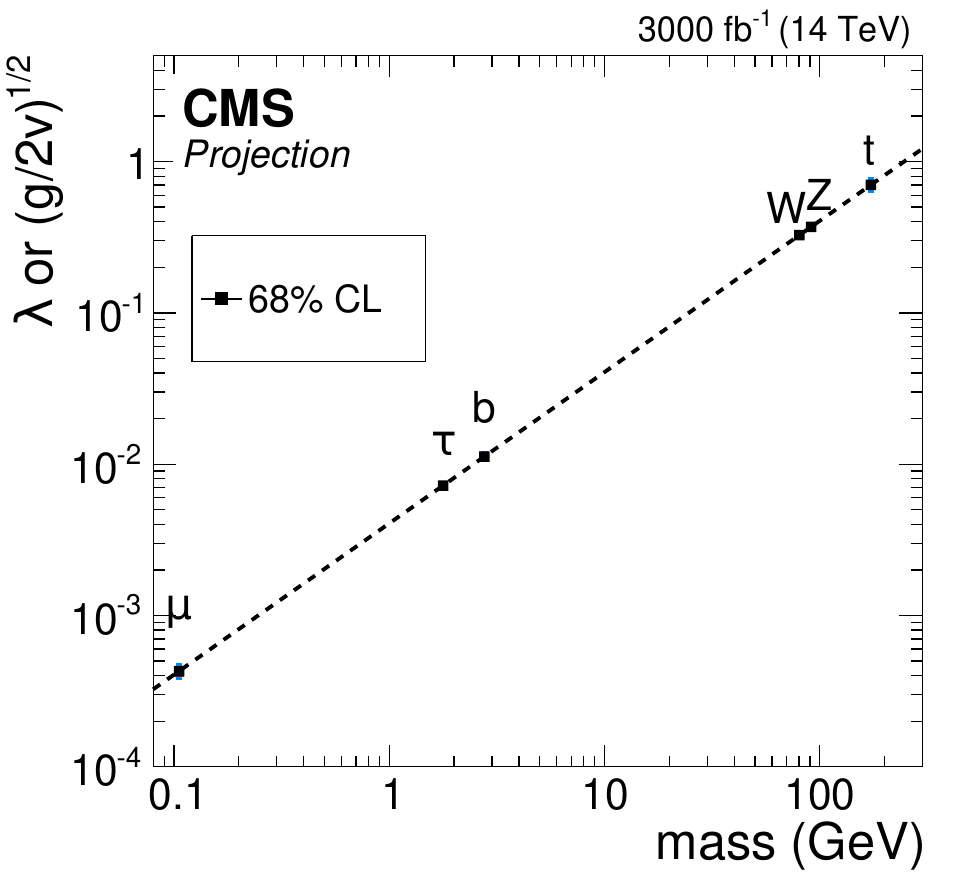
\includegraphics[width =0.7\linewidth]{Figures/Detector/HGCAL/Misc/high_lumi_higgs_couplings.png}\hfill
\caption[The expected precision of Higgs boson coupling measurements at the HL-LHC.]{The expected precision of Higgs boson coupling measurements as a function of particle mass, projected by the end of the HL-LHC operation. Figure taken from Ref~\cite{CMS_phase2_TDR}.}
\label{fig:cms_high_lumi_couplings}
\end{figure}
%could compare a couple with current measurements maybe


\subsection{The High Granularity Calorimeter}

The current technologies used in the CMS endcap calorimeters were designed to operate up to an integrated luminosity of ${\approx}500~\mathrm{fb}^{-1}$, and are thus unable to withstand the considerably higher particle fluxes expected at the HL-LHC. The requirement of radiation tolerance drives the CMS endcap upgrade project, which will see both the EE and HE subsystems replaced by a single, unified sampling calorimeter, comprising both electromagnetic (CE-E) and hadronic (CE-H) sections. Figure~\ref{fig:cms_HGCAL} shows the calorimeter design, which covers the range $1.5<|\eta|\;<3$. 

Silicon sensors are chosen as the active material for the bulk of the detector upgrade, since they have been demonstrated capable of withstanding the expected radiation doses throughout the entire Phase-2 operation. Their fast response also provides timing capabilities for energy deposits, allowing for a significant reduction in out-of-time PU. The CE-E portion consists of 28 layers of tungsten absorber interleaved with silicon sensors of size $0.5$--$1\mathrm{cm}^{2}$, corresponding to around 26~$X_{0}$ of material. The same silicon sensors instrument the entire front section of the CE-H, which contains 12 brass and copper absorber plates, providing excellent energy containment. The rear CE-H component, which extends the calorimeter depth to around 10~$\lambda_{I}$, is instrumented using a combination of silicon sensors and plastic scintillator tiles. The scintillator-technology is positioned at radii further from the beampipe, such that the radiation induced light-loss is minimised. %unified design results in smaller gap between ECAL and HCAL -> benefits resolution

Both the electromagnetic and hadronic components of the HGCAL feature an unprecedented readout granularity with over 6 million channels~\cite{CMS_phase2_HGCAL}, providing considerable benefits for the particle flow (PF)-based reconstruction of physics objects (see Section~\ref{section:PF}). In the lateral direction, fine segmentation allows for separation of neighbouring showers, improving jet resolution and discrimination against PU clusters. The longitudinal segmentation enables frequent sampling of the shower development, providing good energy resolution for electromagnetic objects, including photons from \Hgg decays. Moreover, the high density of the absorber materials results in laterally compact showers that are well contained, improving the resolution of physics signatures involving boosted jet topologies, such as VBF Higgs boson production. %lateral resolution helps matching to tracks too

\begin{figure}[htbp!]
\centering
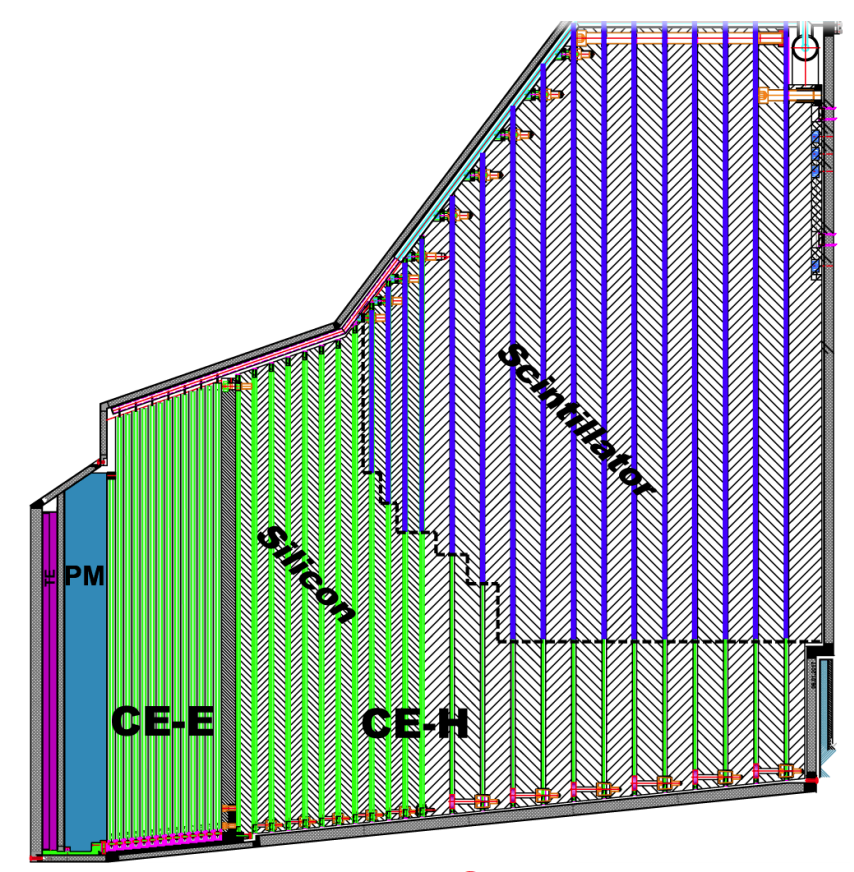
\includegraphics[width =0.5\linewidth]{Figures/Detector/HGCAL/Misc/HGCAL.png}\hfill
\caption[The CMS High Granularity Calorimeter.]{A cut-away section showing the structure of the HGCAL sampling calorimeter. The HGCAL is divided into an initial electromagnetic section, instrumented with a tungsten absorber and silicon readout , and a hadronic section, which uses brass absorbers instrumented with both silicon sensors and plastic scintillator tiles. These components are positioned behind an additional moderator (PM), which reduces the neutron flux penetrating the electromagnetic section. Figure adapted from Ref~\cite{CMS_phase2_HGCAL}.}%purple is a timing layer which helps remove PU
\label{fig:cms_HGCAL}
\end{figure}



\subsection{The HGCAL L1T}

Alongside detector upgrades, a complete replacement of the Level-1 and High-Level Trigger is planned for Phase-2, designed to maintain the trigger efficiency despite the higher luminosity environment. Improvements to front-end electronics and the data acquisition system are expected to increase the L1T latency to 12.5~$\mu\mathrm{s}$, with an allowed total event rate of 750~kHz~\cite{CMS_phase2_L1T}. As a result, more granular information may be exploited to inform L1T decisions, including, for the first time, readout from the tracker system. Tracking information in particular will be crucial in preventing unacceptably high trigger rates, while also allowing for particle flow capabilities at Level-1. An increased latency also enables reconstruction and identification of higher-level objects using more complex selection, including machine learning techniques that could considerably improve trigger efficiencies. These algorithms may be realised through recent advancements in customised, re-programmable electronics known as Field Programmable Gate Arrays, which are expected to bear much of the computational load at Level-1.

Although the L1T system is not fully defined, the envisaged menu will reconstruct a wide variety of objects in order to support a diverse physics programme. This includes triggers targeting single Higgs and promising di-Higgs channels including, for example, $\mathrm{HH}\rightarrow bb\gamma\gamma$; paths supporting B-physics signals that will utilise soft lepton triggers; and triggers targeting large \met signatures typically associated with searches for supersymmetric particles~\cite{CMS_phase2_L1T}.
Many trigger paths at the L1T will require excellent identification of EM showers produced by single electrons or photons ($e/\gamma$), despite the high pileup conditions. The $e/\gamma$ ID algorithms are currently informed by calorimeter information, although studies incorporating track information are also ongoing.

To produce quantities that describe calorimeter deposits for use in the trigger, neighbouring silicon sensors are first grouped into so-called trigger cells (TCs), with a granularity of around 4~$\mathrm{cm}^{2}$. To reduce computational resources, only half of the CE-E layers are used to construct TCs; this is, however, 500 times more granular than the corresponding system used throughout Run 2. The TCs are then sent to backend electronics, which rely on FPGA technologies, and amongst other duties, perform basic clustering of TCs. The clustering is similar to that described in Section~\ref{section:PF}, and can be divided into two steps. The first step defines \textit{seeds} around which 2D clusters can be built. Seeds are defined as TCs with energy above some local, position-dependent maxima. The second step attaches TCs to seeds, provided they are within some geometric neighbourhood. Information from each 2D cluster is then combined depth-wise across layers to form 3D clusters. The position of a cluster is defined as the energy-weighted centre of all TC's in the final cluster, while the energy is defined using TCs within some limited distance from the core, as a compromise between shower containment and contamination from PU. Several other cluster properties describing the shower profile are computed, serving as input to various identification algorithms, including the $e/\gamma$ ID deployed in the HGCAL.

\subsection{Electron and photon identification at the L1T}

The nominal strategy for $e/\gamma$ ID within the HGCAL uses BDT-based classifiers trained to separate clusters resulting from $e/\gamma$ deposits against those resulting from PU. Since observables in electron and photon identification evolve rapidly with $\eta$, two decision trees are trained: one pertaining to a lower $\eta$ region, $1.5 < |\eta|\; \leq 2.7$, the other to a higher eta region, $2.7 < |\eta|\; \leq 3.0$. Given that the shower properties in the HGCAL are similar between photons and electrons, in practice, BDTs are trained only on electron clusters, simulated within a 200~PU event environment. The benchmark pileup per bunch crossing of 200 is chosen instead of the expected value of 140, since the HL-LHC has the ability to deliver 50\% higher values of instantaneous luminosity. %The algo's should also be robust to different PUs!
Signal clusters used for training are defined as those consistent with originating from a generator-level electron, by requiring each cluster to be within a cone of radius $\Delta R < 0.2$ relative to the generator-level electron. Electron clusters must also pass a minimum $p_{\mathrm{T}}$ threshold of 10 GeV. The simulated background comprises all clusters with $p_{\mathrm{T}} > 20$ GeV which are not matched to a generator-level electron. 

%Inputs variables (compatible with FW)
The BDT is implemented using the XGBoost~\cite{xgboost} python library, a gradient boosting package optimised for large datasets. The model is trained on 70\% of the total dataset, with the remaining 30\% withheld for performance evaluation. Nine input features describing both the lateral and longitudinal cluster profile are considered in training, including:

\begin{itemize}
    \item the ratio between the cluster energy deposited in the CE-H to that deposited in the CE-E, $H/E$; %long
    \item the first layer in the cluster to contain an energy deposit above a minimum threshold;%long
    \item the length of the cluster, defined as the difference between the first and last layers that contain energy deposits above threshold; %long
    \item the core cluster length, defined as the maximum number of layers with consecutive energy deposits; %long
    \item the energy weighted RMS of the $\rho$, $\eta$, $\phi$, and $z$ co-ordinates of the cluster TCs, $\sigma_{\rho\rho}$,  $\sigma_{\eta\eta}$, $\sigma_{\phi\phi}$, and $\sigma_{zz}$ respectively, defined for a generic trigger cell co-ordinate, $x$, as
    
    \begin{equation}
            {\rm{Weighted}\,\,\rm{RMS}}(x) = \sqrt{\frac{1}{E_{\rm{tot}}}\sum^{N_{\rm{TC}}}_{i} E_i (x_i-\langle x \rangle)^2},
    \end{equation}
    where $i$ enumerates trigger cells, of which there are $N_{\mathrm{TC}}$, each with energy $E_i$ and co-ordinate $x_i$. The quantity $\langle x \rangle$ is the energy weighted mean of $x$ over all TCs, and $E_{\rm{tot}}$ is the total energy obtained from the sum over all TCs; and %<p> = 1/Etot * (sum E_i * p_i)
    \item the cluster centre, in z-coorindates, $\langle z \rangle$. %lat
\end{itemize}

\noindent The majority of inputs inputs to both classifiers show good separation between signal and background clusters. In particular, Figure~\ref{fig:HGCAL_egid_inputs} (left) shows the distribution of $\sigma_{\eta\eta}$, describing the lateral shower spread in $\eta$, which is typically narrower for $e/\gamma$ clusters. Also shown in Figure~\ref{fig:HGCAL_egid_inputs} (right) is the ratio $H/E$. Events associated with signal clusters typically deposit the majority of their energy in the CE-E, resulting in small values of H/E in comparison to PU clusters, where the energy deposited extends out to later layers of the CE-H.

\begin{figure}[htbp!]
\centering
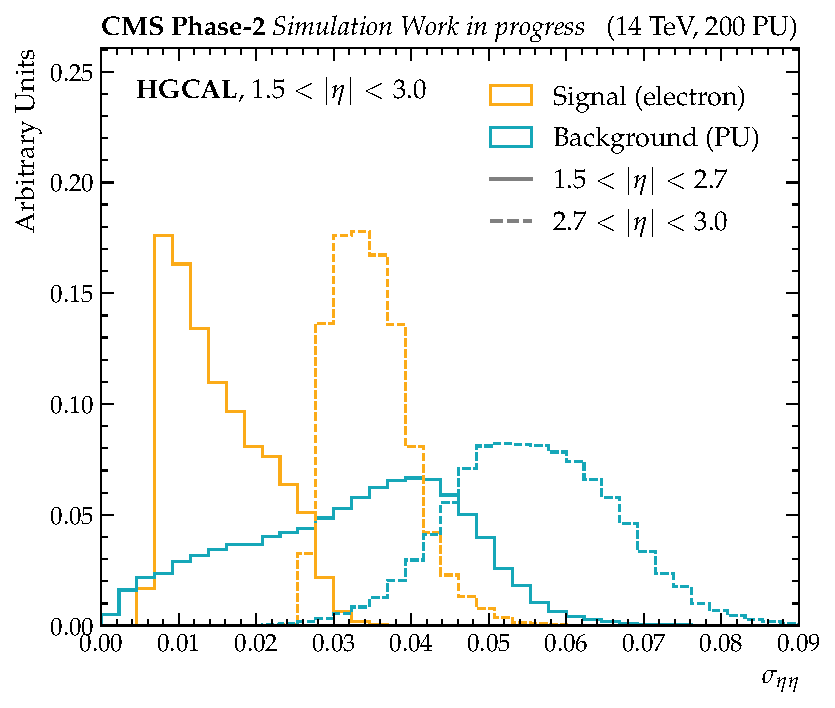
\includegraphics[width=0.49\linewidth]{Figures/Detector/HGCAL/InputsOutputs/sig_vs_bkg_cl3d_seetot_both_eta.pdf}\hfill% 
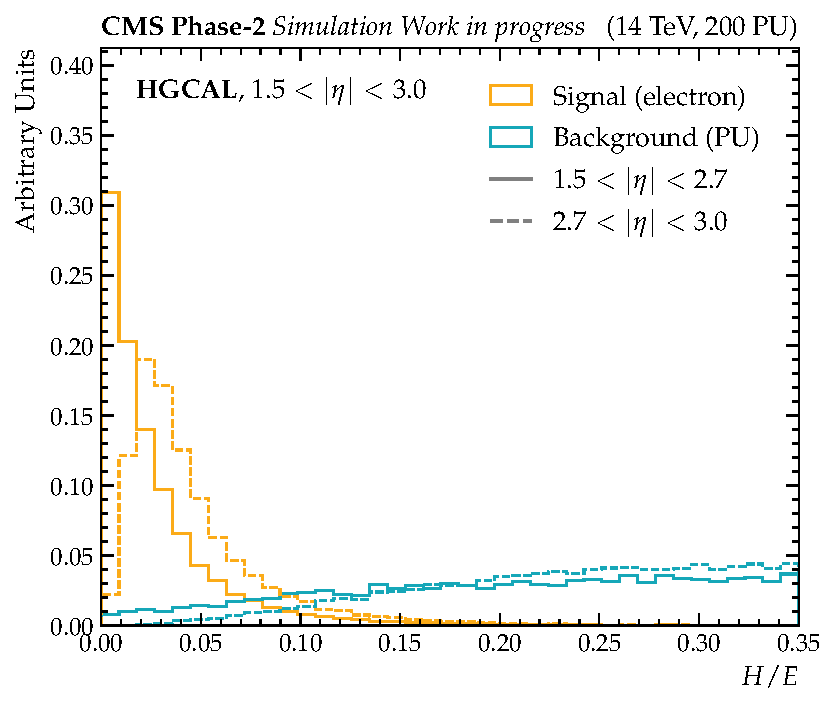
\includegraphics[width=0.49\linewidth]{Figures/Detector/HGCAL/InputsOutputs/sig_vs_bkg_cl3d_hoe_both_eta.pdf}
\caption[Selected inputs to the HGCAL L1T $e/\gamma$ identification BDTs.]{Selected inputs to the HGCAL $e/\gamma$ ID BDTs, shown for simulated single electron (signal) and pileup (background) clusters. The outcome of the classifier will inform decisions in the CMS Phase-2 L1T. Events are separated into the two $\eta$ regions in which a model is trained, and normalised such that the integral of each histogram is unity.  Left: the energy weighted RMS of the $\eta$ co-ordinate of the cluster TCs. Right: the cluster energy deposited in the CE-H divided by that deposited in the CE-E.}
\label{fig:HGCAL_egid_inputs}
\end{figure}

%Performance
The performance of each BDT is evaluated using the area under the associated ROC curve. The output score distributions used to generate performance curves are shown for each classifier in Figure~\ref{fig:HGCAL_egid_output}. The distributions for signal and pileup events are extremely well separated, resulting in ROC curves with large areas shown in Figure~\ref{fig:HGCAL_egid_ROC}. The performance is summarised for each classifier using thresholds on the output score, known as \textit{working points}, which correspond to various signal efficiency benchmarks. For the classifier trained in the lower $\eta$ region, a benchmark signal efficiency of 97.5\% is chosen, while for the higher $\eta$ region, where the number of pileup interactions per bunch crossing is higher, a value of 90.0\% is preferred. These correspond to high background rejection rates of 99.36\% and 99.69\% respectively, where background rejection is defined as one minus the background efficiency.

\begin{figure}[htbp!]
\centering
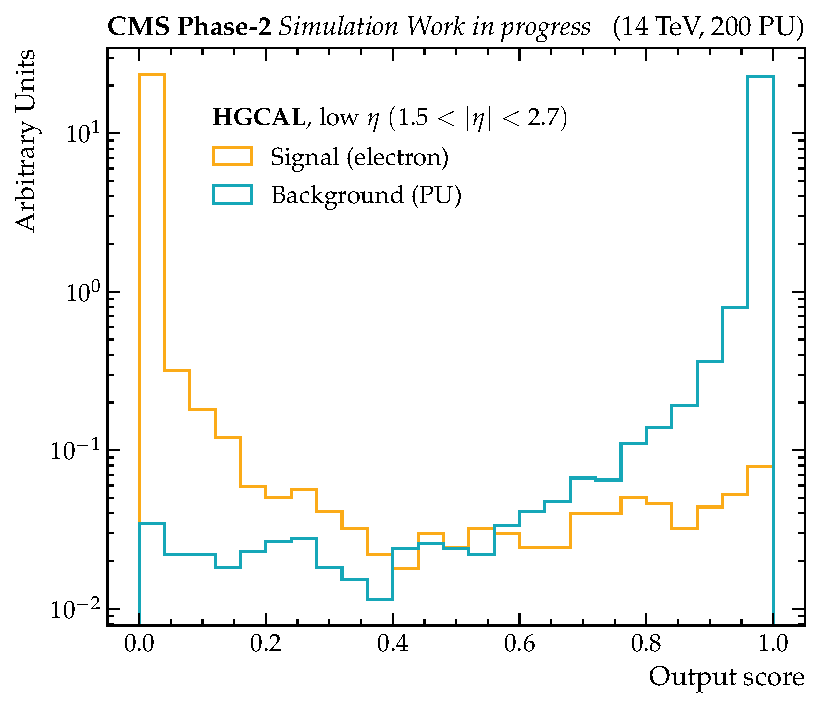
\includegraphics[width=0.49\linewidth]{Figures/Detector/HGCAL/InputsOutputs/EGID_output_score_low_eta.pdf}\hfill% 
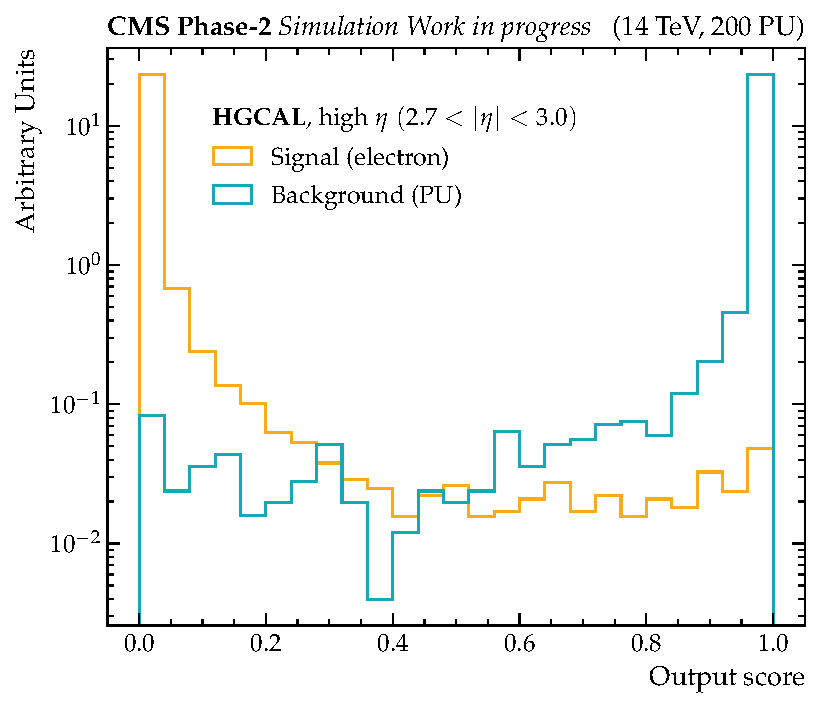
\includegraphics[width=0.49\linewidth]{Figures/Detector/HGCAL/InputsOutputs/EGID_output_score_high_eta.pdf}
\caption[Output score distributions for the HGCAL L1T $e/\gamma$ identification BDTs.]{Output score distributions for the HGCAL $e/\gamma$ ID BDTs for simulated electron (signal) and pileup (background) clusters. The BDT trained in the lower $\eta$ region ($1.5 < |\eta|\; \leq 2.7$) is shown on the left, while the BDT trained in the higher $\eta$ region ($2.7 < |\eta|\; \leq 3$) is shown on the right. Output scores are shown for the test set, containing 30\% of the total events. The output score distributions are well separated between signal and background clusters.}
\label{fig:HGCAL_egid_output}
\end{figure}

\begin{figure}[htbp!]
\centering
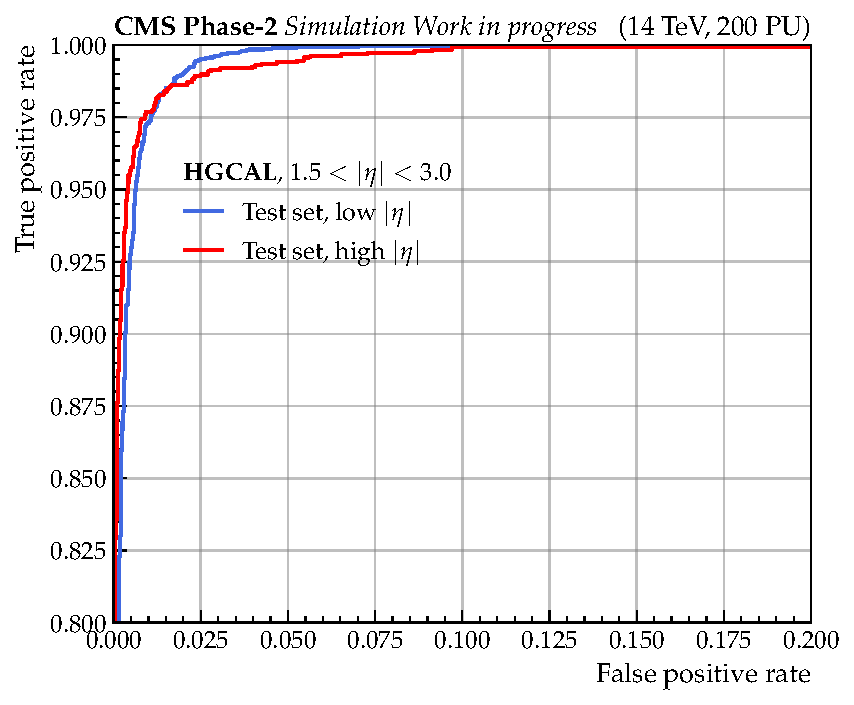
\includegraphics[width=0.54\linewidth]{Figures/Detector/HGCAL/InputsOutputs/EGID_ROC_curve_all_eta.pdf}\hfill% 
\caption[The ROC curves for the HGCAL L1T $e/\gamma$ identification BDTs.]{The ROC curves for the two $e/\gamma$ identification BDTs used in the HGCAL L1T, separated by $\eta$ region. The curve is produced using events from the test set, comprising 30\% of the total events. For both classifiers, the TPR remains high even at low FPR values, resulting in large areas under the curve.}
\label{fig:HGCAL_egid_ROC}
\end{figure}

All clusters passing the $e/\gamma$ ID requirements are then promoted to calorimeter-only $e/\gamma$ candidates, with the energy determined using the CE-E layers. Clusters within the tracker acceptance are considered for track-matching, using track-finder trigger primitives with \pt$>10$~GeV that have been propagated to the calorimeter surface. These electron-like objects are also corrected for bremsstrahlung losses by merging neighbouring low energy deposits passing the $e/\gamma$ ID into the highest energy cluster. Photon deposits are identified as showers without a matching track. Finally, the resulting objects are compared against the L1T trigger menu, with events receiving an ``accept" signal sent to detector read-out electronics.

\subsection{Firmware constraints and feature selection}
\label{subsec:feature_selection}

The $e/\gamma$ ID algorithms for the HGCAL will ultimately be realised in firmware, and must operate in real time within the constraints of the L1T system. The entire HCAL output should be received by the central L1T system within 5~$\mu\mathrm{s}$, which requires the latency for clustering and property evaluation to be less than 1~$\mu\mathrm{s}$. Although the exact cluster properties to be evaluated are not completely defined, it is expected that they should require between 128 and 416 bits of memory, in order to remain within the total HGCAL bandwidth allocation of 60,000 bits per endcap, in each bunch crossing~\cite{CMS_phase2_HGCAL}. In order to be compatible with these constraints, the $e/\gamma$ ID must use as few computational resources as possible; importantly, it must be both quick to evaluate and memory efficient. %mem requirements on page 51 of HGCAL TDR and L1T TPG section

One strategy to reduce the computational complexity is to truncate the number of input features provided to the classifier. Boosted decision trees trained with fewer features typically result in more simple base learners, resulting in quicker evaluation during online inference. In addition, removing quantities that do not significantly contribute to performance prevents redundant variables being constructed in firmware, reducing memory requirements. Naturally, removing many features will eventually degrade the performance of the classifier; the objective, therefore, is to remove a maximum number of features, whilst still maintaining reasonable discrimination power against PU clusters. 

Typical feature reduction algorithms aim to remove inputs that are deemed to contribute little predictive power to the overall model. To quantify the importance of a feature, the notion of Shapley values is used~\cite{SHAPTheory,SHAP}. A Shapley value measures the contribution of a feature value, for a given event, to the difference between the prediction for that event and the mean prediction over all events\footnote{For a feature value $x_{i}$, the Shapley value is $x_{i}$'s marginal contribution to the predicted value for event $i$ minus the mean prediction over all events, averaged over all possible permutations (or \textit{coalitions}) of the features under consideration.}. Values with large magnitude are associated with predictions that strongly support a given class. Since a Shapley value is computed at the per-event level, to obtain a single measure of importance for each feature, the mean of the absolute Shapley values is taken. Figure~\ref{fig:HGCAL_shap_pie_charts} shows the fractional breakdown of mean absolute Shapley values for each variable, for both $e/\gamma$ ID BDTs. In both models, around 75\% of the total importance is attributed to just two inputs, namely $H/E$ and $\sigma_{\rho\rho}$. For the lower $\eta$ classifier, the remaining feature importance values are distributed semi-evenly, with the exception of the three least important features which contribute very little. For the higher $\eta$ classifier, the $\sigma_{\phi\phi}$ quantity contains the majority of the remaining importance, meaning around 85\% can be attributed to only three inputs. Although these asymmetric importance distributions highlight an opportunity for variable pruning, it should be noted that the relative importance can also shift between updates to the feature set.
%The sum of Shapley values over all features gives the difference between the mean prediction and the prediction for this event being considered.

\begin{figure}[htbp!]
\centering
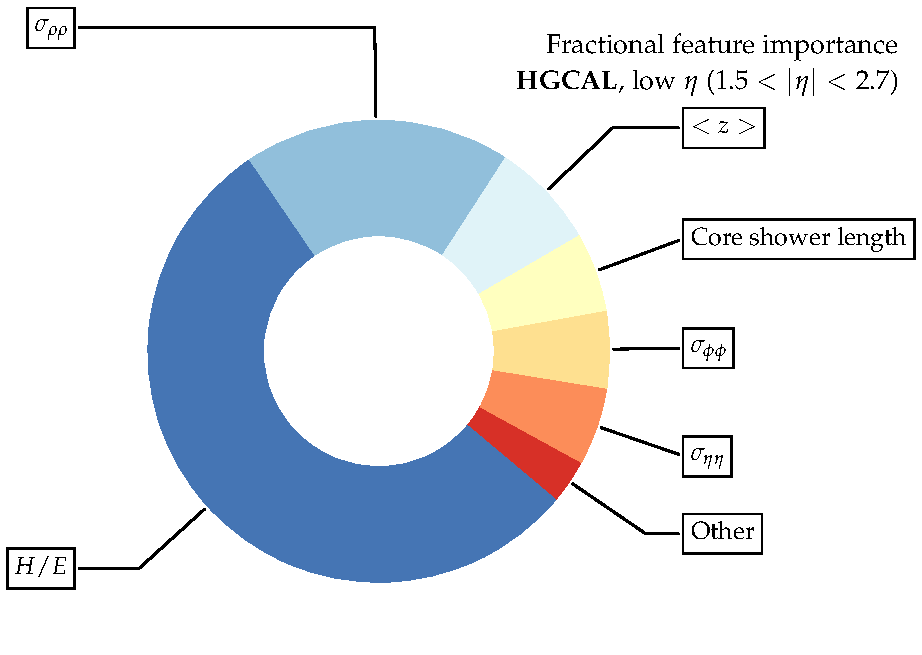
\includegraphics[width=0.49\linewidth]{Figures/Detector/HGCAL/featureSelection/pie_chart_low_eta.pdf}\hfill% 
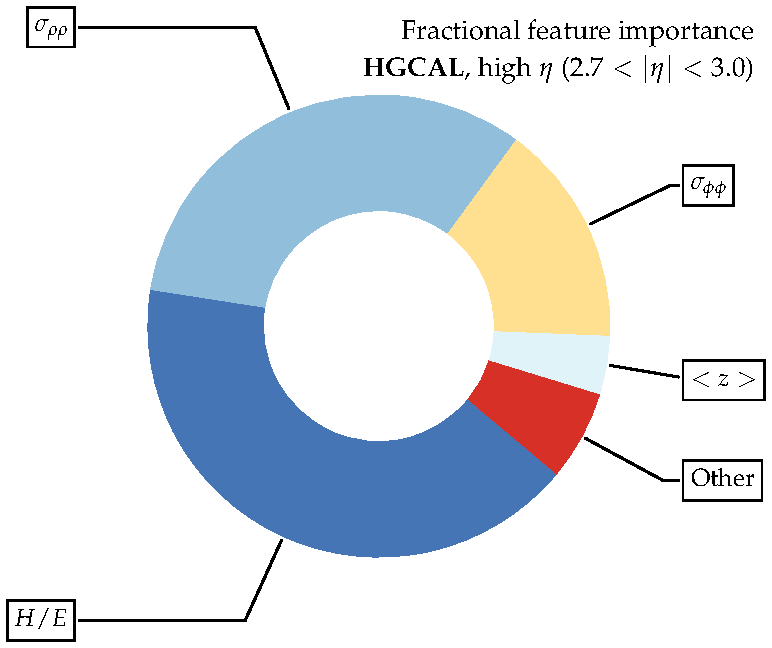
\includegraphics[width=0.39\linewidth]{Figures/Detector/HGCAL/featureSelection/pie_chart_high_eta.pdf}
\caption[The feature importance for inputs to the HGCAL L1T $e/\gamma$ identification BDTs.]{The fractional mean absolute Shapley values for each input feature to the HGCAL L1T $e/\gamma$ ID BDTs. The model trained in the lower $\eta$ region is shown on the left, while the model trained in the higher $\eta$ region is shown on the right. For both models, the quantities $H/E$ and $\sigma_{\rho\rho}$ are responsible for approximately 75\% of the total feature importance scores. Variables with small importance are shown inclusively by the segment labelled ``other".}
\label{fig:HGCAL_shap_pie_charts}
\end{figure}

One common feature reduction technique, known as \textit{sequential backward selection} (SBS), removes one feature per iteration, starting from the full set of (nine) features. At each training step, the feature with the smallest Shapley value is dropped from the set. The process is repeated until a termination criteria is reached, which is typically a lower performance threshold. The model is re-trained between updates to the feature set, to account for shifts in importance between models. The resulting performance when applied to each $e/\gamma$ ID BDT, measured using the area under the ROC curve, is summarised for each step in the algorithm in Figure~\ref{fig:HGCAL_egid_SBS}. To obtain an estimate of the uncertainty, the model is evaluated many thousands of times on bootstrapped samples of the test set, where events are drawn at random and with replacement. The average ROC AUC is taken as the central value, with the standard deviation of the scores used to estimate the uncertainty on the mean. 

For the classifier trained in the low $\eta$ region, the performance is unaffected up to the removal of three variables. This could be expected from the importance distribution in Figure~\ref{fig:HGCAL_shap_pie_charts}, where the three least important variables contribute very little to the overall model importance. A small degradation is seen when removing additional variables, although the loss in background rejection efficiency is modest; removing five variables, which would decrease the memory required for cluster properties by more than one half, still maintains a background rejection efficiency of 99.22\%, at the usual 97.5\% signal efficiency benchmark.  Results for the BDT trained in the higher $\eta$ region are also encouraging, with the original performance maintained up to the removal of six variables. This is again expected from Figure~\ref{fig:HGCAL_shap_pie_charts}, where the majority of the feature importance can be attributed to only a handful of inputs. At the benchmark signal efficiency of 90.0\%, removing six variables maintains a background rejection rate of 99.67\%, comparable to the nominal model trained with all features.


\begin{figure}[htbp!]
\centering
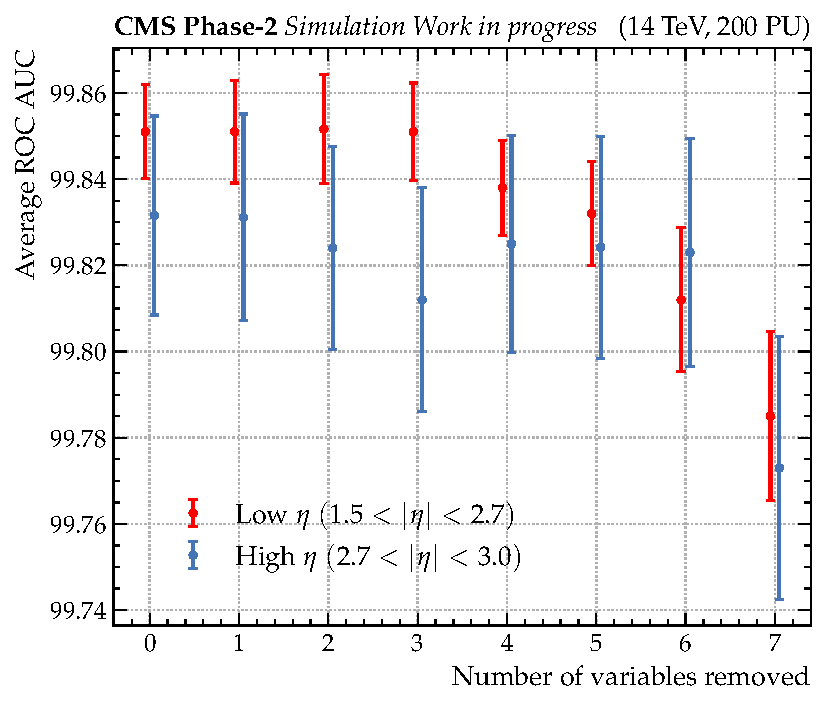
\includegraphics[width=0.49\linewidth]{Figures/Detector/HGCAL/featureSelection/ROCs_low_high.pdf}\hfill% 
\caption[The evolution of BDT performance with the number of variables used within the HGCAL L1T $e/\gamma$ identification BDTs.]{The evolution of performance with decreasing number of variables for the HGCAL L1T $e/\gamma$ ID BDTs. Performance is measured using the area under the ROC curve, averaged across many bootstrapped samples of the test set, with the standard deviation used to estimate the uncertainty on the mean. The performance of the low $\eta$ BDT, shown in red, degrades slightly upon removal of more than three variables, and noticeably worsens once six and seven variables have been removed. Performance of the model trained in the high $\eta$ region, shown in blue, is maintained up to the removal of six input variables. A small amount of overtraining results in larger uncertainties on the average ROC score when compared with the corresponding low $\eta$ model.}
\label{fig:HGCAL_egid_SBS}
\end{figure}

Although promising, feature reduction through the SBS algorithm may not yield optimal feature sets at each iteration. The algorithm is \textit{greedy}, given that it can only assess the most important feature in the current training, and cannot look ahead to future iterations where the distribution of importances may change. Therefore, extensions to this work may consider alternative approaches using more holistic algorithms. Studies using more sophisticated methods, for example the Boruta feature selection algorithm~\cite{Boruta}, have shown similar results to that of SBS. Other approaches using evolutionary algorithms could also be applied with success. In addition, the complication of training two separate BDTs, one pertaining to each region in $\eta$, has effectively been ignored, given that the top ranking features are similar between models. With the possible advent of new cluster properties in future L1T design iterations, the feature importance rankings could differ significantly between models. This may require features that are redundant in one classifier still being computed for use in the other, resulting in larger memory requirements. Overall, however, feature reduction in the $e/\gamma$ ID appears a viable method to reduce the computational requirements associated with online model implementation and inference in the HGCAL L1T. The technique is applicable not only to BDTs, but to any such machine learning model that may eventually be deployed. Thus far, studies have aimed at removing a maximum number of features while maintaining close to the original performance; the final realistic constraints that will ultimately inform the choice of model will only be available once the L1T architecture for Phase-2 operation is decided upon. 

\section{Summary}

The CMS detector detector is one of two general-purpose detectors situated on the LHC ring, aiming to measure the properties of hadron collisions. Its design centres around a 3.8~T solenoidal magnet and comprises an inner tracker, electromagnetic and hadronic calorimeters, and muon system. Together, these components allow for reconstruction of a wide range of physics objects with high efficiency, including electrons, photons, muons, and jets, over a range of momenta and angles. In addition, the two-level trigger system allows for events of interest to be selected with high efficiency, while maintaining a tolerable readout rate. Upgrade projects for the CMS detector in preparation for the high luminosity Phase-2 operation of the LHC include a new endcap calorimeter, which will inform the L1T decision. A key component of the trigger menu will be identification of $e/\gamma$ objects against pileup clusters, to which end, dedicated BDT-based classifiers are trained. The classifiers will be evaluated online, and must therefore adhere to the latency and bandwidth constraints associated with the L1T architecture. Various techniques to reduce the computational resources of the $e/\gamma$ ID are being considered, including reducing the input feature set provided to online models. These feature selection algorithms have been demonstrated to reduce the cluster memory requirements, while also maintaining excellent rejection of pileup clusters.
    